\documentclass[11pt,a4paper]{article}

\usepackage[utf8]{inputenc}
\usepackage[spanish]{babel}
\usepackage{amsmath}
\usepackage{float}
\usepackage{amsfonts}
\usepackage{amssymb}
\usepackage{makeidx}
\usepackage{graphicx}
\usepackage{lmodern}
\usepackage{kpfonts}
\usepackage{wrapfig}
\usepackage{caption}
\usepackage{subcaption}
\usepackage{booktabs}
\usepackage[nottoc,numbib]{tocbibind} %agrega la bibliografia al índice.
\usepackage[font={small,it}]{caption}
%\usepackage{fourier}
\usepackage[left=2cm,right=2cm,top=2cm,bottom=2cm,headheight=13.6pt]{geometry}
\usepackage{fancyhdr}
\usepackage{multirow}
\pagestyle{fancy}


%Para los gráficos en general, con las tablas...¡Ja!, arreglate.
%\begin{figure}[h!]
%\centering
%\includegraphics[width=0.7\textwidth]{} %nombre de la imagen, incluirla en el mismo directorio que este archivo.
%\caption*{} %rótulo, el asterico elimina la numeración automática. 
%\label{fig:} % para luego referirse con \ref{fig:}
%\end{figure}


\begin{document}


%%%%%%%%%%%%%%%%%%%%%%%%%%%%%%%%%%%%%%%%%%%%%%%%%%%%%%%%%%%%%%%%%%%%%%%%%%%%%%%%%%%%%%%%%%%%%%%%%%%%%%%%%%%%%%%%%%%%%%%%%%%%%%%%%
% 	TÍTULO
%%%%%%%%%%%%%%%%%%%%%%%%%%%%%%%%%%%%%%%%%%%%%%%%%%%%%%%%%%%%%%%%%%%%%%%%%%%%%%%%%%%%%%%%%%%%%%%%%%%%%%%%%%%%%%%%%%%%%%%%%%%%%%%%%

%%%%%%%%%%%%%%%%%%%%%%%%%%%%%%%%%%%%%%%%%
% University Assignment Title Page 
% LaTeX Template
% Version 1.0 (27/12/12)
%
% This template has been downloaded from:
% http://www.LaTeXTemplates.com
%
% Original author:
% WikiBooks (http://en.wikibooks.org/wiki/LaTeX/Title_Creation)
%
% License:
% CC BY-NC-SA 3.0 (http://creativecommons.org/licenses/by-nc-sa/3.0/)
% 
% Instructions for using this template:
% This title page is capable of being compiled as is. This is not useful for 
% including it in another document. To do this, you have two options: 
%
% 1) Copy/paste everything between \begin{document} and \end{document} 
% starting at \begin{titlepage} and paste this into another LaTeX file where you 
% want your title page.
% OR
% 2) Remove everything outside the \begin{titlepage} and \end{titlepage} and 
% move this file to the same directory as the LaTeX file you wish to add it to. 
% Then add \input{./title_page_1.tex} to your LaTeX file where you want your
% title page.
%
%%%%%%%%%%%%%%%%%%%%%%%%%%%%%%%%%%%%%%%%%

%----------------------------------------------------------------------------------------
%	PACKAGES AND OTHER DOCUMENT CONFIGURATIONS
%----------------------------------------------------------------------------------------

%\documentclass[12pt]{article}
%\usepackage[utf8]{inputenc}
%\usepackage[spanish]{babel}
%\begin{document}

\begin{titlepage}

\newcommand{\HRule}{\rule{\linewidth}{0.5mm}} % Defines a new command for the horizontal lines, change thickness here

\center % Center everything on the page
 
%----------------------------------------------------------------------------------------
%	HEADING SECTIONS
%----------------------------------------------------------------------------------------

\textsc{\Huge Universidad de Buenos Aires}\\[0.5cm]
\textsc{\LARGE Facultad de Ciencias Exactas y Naturales}\\[0.5cm] % Name of your university/college
\textsc{\Large Departamento de Física}\\[0.25cm] % Major heading such as course name

\begin{figure}[h]
  \centering
  
\includegraphics[scale=0.15]{Logo_DF}
  \\[0.5cm]
\end{figure}

\textsc{\large Laboratorio 3}\\[0.25cm] % Minor heading such as course title

%----------------------------------------------------------------------------------------
%	TITLE SECTION
%----------------------------------------------------------------------------------------

\HRule \\[0.4cm]
{ \huge \bfseries Transitorio y tiempo caracteristico de circuitos}\\[0.2cm] % Title of your document
\HRule \\[1cm]
 
%----------------------------------------------------------------------------------------
%	AUTHOR SECTION
%----------------------------------------------------------------------------------------

\begin{minipage}{0.4\textwidth}
\begin{center} \large
\emph{Autores:}\\
\textsc{Andreu}, Gonzalo\\ % Your name
\textsc{Malpartida}, Bryan\\ % Your name
\textsc{Pugliese}, Facundo\\ % Your name


\end{center}
\end{minipage}
~ \\[1.25cm]
%\begin{minipage}{0.4\textwidth}
%\begin{flushright} \large
%\emph{Supervisor:} \\
%Dr. James \textsc{Smith} % Supervisor's Name
%\end{flushright}
%\end{minipage}\\[4cm]

% If you don't want a supervisor, uncomment the two lines below and remove the section above
%\Large \emph{Author:}\\
%John \textsc{Smith}\\[3cm] % Your name

%----------------------------------------------------------------------------------------
%	DATE SECTION
%----------------------------------------------------------------------------------------

%\vspace{\fill}


{\large 17 de Febrero de 2016}\\[1.75cm] % Date, change the \today to a set date if you want to be precise

%----------------------------------------------------------------------------------------
%	SUMMARY SECTION: No más de 15 renglones, no te zarpes
%----------------------------------------------------------------------------------------

\begin{center}
\large{\textbf{Resumen}}

\small{El objetivo del siguiente trabajo fue caracterizar circuitos RC, RL y RCL. 

Para los dos primeros casos, los circuitos RC y RL, se buscó determinar el tiempos característico de cada uno variando los parámetros de cada sistema. Ademas de poder observar los fenómenos particulares en estos sistemas, como la carga y descarga del capacitor y la disminución de la corriente debido a la inductancia, utilizando una fuente de alimentación que emitía señales cuadradas y osciloscopio como instrumento de medición.

Por otro lado, el estudio del circuito RCL se centró en la observación de los comportamientos que tiene el mismo para distintos parámetros del sistema. Para ellos se obtenían teóricamente los valores necesarios de cada parámetro para luego $settear$ los elementos del circuito y comprobar que la evolución del sistema cumpliese el modelo teórico. Dichas observaciones se obtuvieron nuevamente utilizando una fuente de señal cuadrada y un osciloscopio.

Finalmente, el método resulto eficiente a la hora de comprobar las ecuaciones referidas al circuito RC y, en menor medida, al circuito RL. En el caso del circuito RCL, pudieron analizarse los casos extremos de comportamiento, pero no el comportamiento borde debido a lo fino del mismo.} % ACA VA EL RESUMEN

\end{center}


%----------------------------------------------------------------------------------------
%	LOGO SECTION
%----------------------------------------------------------------------------------------

%\includegraphics{Logo}\\[1cm] % Include a department/university logo - this will require the graphicx package
 
%----------------------------------------------------------------------------------------

\vfill % Fill the rest of the page with whitespace

\end{titlepage}
%\end{document} %incluir en el mismo directorio que este archivo. Equivalente a un copiar-pegar, nada de andar diciendo \begin{document} en la portada. Dejar el nombre de Caratula a la caratula.

%%%%%%%%%%%%%%%%%%%%%%%%%%%%%%%%%%%%%%%%%%%%%%%%%%%%%%%%%%%%%%%%%%%%%%%%%%%%%%%%%%%%%%%%%%%%%%%%%%%%%%%%%%%%%%%%%%%%%%%%%%%%%%%%%
% 	ENCABEZADO Y PIE DE PÁGINA.
%%%%%%%%%%%%%%%%%%%%%%%%%%%%%%%%%%%%%%%%%%%%%%%%%%%%%%%%%%%%%%%%%%%%%%%%%%%%%%%%%%%%%%%%%%%%%%%%%%%%%%%%%%%%%%%%%%%%%%%%%%%%%%%%%

\lhead{}
\chead{}
\rhead{Laboratorio 3}
\lfoot{}
\cfoot{}
\rfoot{\thepage}
\renewcommand{\headrulewidth}{1pt}
\renewcommand{\footrulewidth}{1pt}


%%%%%%%%%%%%%%%%%%%%%%%%%%%%%%%%%%%%%%%%%%%%%%%%%%%%%%%%%%%%%%%%%%%%%%%%%%%%%%%%%%%%%%%%%%%%%%%%%%%%%%%%%%%%%%%%%%%%%%%%%%%%%%%
% Página en blanco. Cita, agradecimiento, dedicación, lo que sea pero que sea algo.
%%%%%%%%%%%%%%%%%%%%%%%%%%%%%%%%%%%%%%%%%%%%%%%%%%%%%%%%%%%%%%%%%%%%%%%%%%%%%%%%%%%%%%%%%%%%%%%%%%%%%%%%%%%%%%%%%%%%%%%%%%%%%%%


%%%%%%%%%%%%%%%%%%%%%%%%%%%%%%%%%%%%%%%%%%%%%%%%%%%%%%%%%%%%%%%%%%%%%%%%%%%%%%%%%%%%%%%%%%%%%%%%%%%%%%%%%%%%%%%%%%%%%%%%%%%%%%%%%
% 	ÍNDICE
%%%%%%%%%%%%%%%%%%%%%%%%%%%%%%%%%%%%%%%%%%%%%%%%%%%%%%%%%%%%%%%%%%%%%%%%%%%%%%%%%%%%%%%%%%%%%%%%%%%%%%%%%%%%%%%%%%%%%%%%%%%%%%%%%

%\tableofcontents %compilar dos o tres veces para verlo bien. ¡Todo un índice en unas cuantas letras!
%\newpage

%%%%%%%%%%%%%%%%%%%%%%%%%%%%%%%%%%%%%%%%%%%%%%%%%%%%%%%%%%%%%%%%%%%%%%%%%%%%%%%%%%%%%%%%%%%%%%%%%%%%%%%%%%%%%%%%%%%%%%%%%%%%%%%
% 1. RESUMEN
%%%%%%%%%%%%%%%%%%%%%%%%%%%%%%%%%%%%%%%%%%%%%%%%%%%%%%%%%%%%%%%%%%%%%%%%%%%%%%%%%%%%%%%%%%%%%%%%%%%%%%%%%%%%%%%%%%%%%%%%%%%%%%%

%\section{Resumen}
%\label{sec:resumen}



%%%%%%%%%%%%%%%%%%%%%%%%%%%%%%%%%%%%%%%%%%%%%%%%%%%%%%%%%%%%%%%%%%%%%%%%%%%%%%%%%%%%%%%%%%%%%%%%%%%%%%%%%%%%%%%%%%%%%%%%%%%%%%%
% 2. INTRODUCCIÓN: ecuaciones aquí, luego se las cita.
%%%%%%%%%%%%%%%%%%%%%%%%%%%%%%%%%%%%%%%%%%%%%%%%%%%%%%%%%%%%%%%%%%%%%%%%%%%%%%%%%%%%%%%%%%%%%%%%%%%%%%%%%%%%%%%%%%%%%%%%%%%%%%%

\section{Introducción}\label{sec:intro}
\subsection{El diodo}
El diodo ideal es un componente que permite la circulación de corriente entre sus terminales en un determinado sentido, mientras que la bloquea en el sentido contrario. El funcionamiento del diodo ideal es el de un componente que presenta resistencia nula al paso de la corriente en un determinado sentido, y resistencia infinita en el sentido opuesto.
Mediante el siguiente ejemplo mostrado en la \textbf{figura \ref{fig:Ejemplo}} se pretende mostrar el funcionamiento ideal de un diodo en circuito sencillo.

\begin{figure}[H]

\begin{subfigure}{0.5\textwidth}
\centering
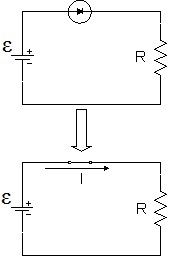
\includegraphics[scale=0.8]{Ejemplo-Funcionamiento-Diodo-Ideal-Polarizacion-Directa}
   \subcaption{Diodo ideal en polarizacion directa.}
   \label{subfig:Pol-Dir}
\end{subfigure}
\begin{subfigure}{0.5\textwidth}
\centering
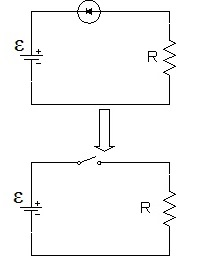
\includegraphics[scale=0.8]{Ejemplo-Funcionamiento-Diodo-Ideal-Polarizacion-Inversa}
   \subcaption{Diodo ideal en polarizacion indirecta.}
   \label{subfig:Pol-Inv}
\end{subfigure}

  \caption{Ejemplo del funcionamiento de un diodo ideal en un circuito simple. La corriente circula en sentido horario para los dos casos.}
   \label{fig:Ejemplo}
\end{figure}

En el circuito de \textbf{figura \ref{subfig:Pol-Dir}}, el diodo permite dicha circulación, ya que la corriente entra por el ánodo, y éste se comporta como un interruptor cerrado. Debido a esto, se produce una caída de tensión en la resistencia, y se obtiene una corriente. En el de la \textbf{figura \ref{subfig:Pol-Inv}}, en cambio, el diodo impide el paso de corriente, comportándose como un interruptor abierto, y la caída de tensión en la resistencia es nula.

Un diodo consta de dos zonas hechas de materiales semiconductores con caracteristicas opuestas. Una zona tiene un exceso de \textit{huecos}, mientras que la otra dispone de electrones en exceso, pero aun asi, en cada zona la carga total es neutra. En el momento mismo de crear dos zonas de diferente concentración de portadores, entra en juego el mecanismo de la difusión. La distribución de cargas formada en la región de la unión provoca un campo eléctrico desde la zona N a la zona P que se opone al movimiento de portadores y que va creciendo conforme pasan más cargas a la zona opuesta hasta que se llega a un equilibrio. En ese momento está ya formado el diodo de unión PN ilustrado en la \textbf{figura \ref{fig:Dif}}, y como resultado del proceso se ha obtenido una zona P y una zona N, ambas semiconductoras, y una zona de agotamiento (deplección) que es no conductora. En ella actúa un campo eléctrico, o bien entre los extremos actúa una barrera de potencial.

\begin{figure}[h]
\centering
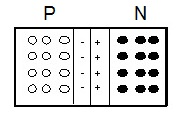
\includegraphics[scale=0.8]{Difusion}
   \caption{Ilustracion de diodo de unio PN}
   \label{fig:Dif}
\end{figure}

El bloque PN  en principio no permite el establecimiento de una corriente eléctrica entre sus terminales puesto que la zona de deplección no es conductora. Sin embargo, si se aplica una tensión positiva en el ánodo mayor que la de la barrera, desaparecera la zona de deplección y el dispositivo conduce de forma que en una primera aproximacion respeta la siguiente ecuacion:

\begin{equation}{\label{Aprox}}
\Delta  V_D = I.R_D\\
\end{equation}

 Por el contrario, al aplicar una tensión positiva a la zona N y negativa a la zona P, se retiran portadores mayoritarios próximos a la unión. Estos portadores son atraídos hacia los contactos aumentando la anchura de la zona de agotamiento, lo cual hace que la corriente debido a los portadores mayoritarios sea nula. Ahora bien, en ambas zonas hay portadores minoritarios que son atraídos hacia la unión creando una corriente inversa, aunque muy inferior que la obtenida en polarización directa. Al aumentar la tensión inversa, llega un momento en que se produce la ruptura de la zona de deplección, al igual que sucede en un material aislante: el campo eléctrico puede ser tan elevado que arranque electrones que forman los enlaces covalentes, originando un proceso de rotura por avalancha y generando una corriente que respeta la ecuacion \eqref{Aprox} pero con una resistencia mayor.

%%%%%%%%%%%%%%%%%%%%%%%%%%%%%%%%%%%%%%%%%%%%%%%%%%%%%%%%%%%%%%%%%%%%%%%%%%%%%%%%%%%%%%%%%%%%%%%%%%%%%%%%%%%%%%%%%%%%%%%%%%%%%%%
% 3. DISPOSITIVO EXPERIMENTAL: armado del modelo, como se midio, consideraciones a la hora de medir.
%%%%%%%%%%%%%%%%%%%%%%%%%%%%%%%%%%%%%%%%%%%%%%%%%%%%%%%%%%%%%%%%%%%%%%%%%%%%%%%%%%%%%%%%%%%%%%%%%%%%%%%%%%%%%%%%%%%%%%%%%%%%%%%

\section{Desarrollo experimental}

Durante esta experiencia se utilizó un generador de funciones de emitir frecuencias con un error relativo del $0,01\%$ en un rango entre $1\mu Hz$ y $5MHz$ cuyo voltaje pico-pico tiene un error relativo del $1\%$ para el rango de voltaje utilizado ($2V-20V$). Además, se utilizó una capacitancia y una resistencia, ambas variables por décadas cuyo error fue a priori desconocido. Usando un multimetro digital se midieron los valores configurados en cada instrumento junto con su error que, para las resistencias, era de la forma $\pm(1\%+2d)$ en el rango utilizado (mayor a $100\Omega$), y para las  capacitancias, $\pm(4\%+3d)$. La resistencia del capacitor resultó despreciable.

Se utilizó un osciloscopio digital, con dos canales de entrada, capaz de medir diferencias de potencial entre las dos terminales que dispone en un rango de 2mV a 5V con un error relativo del $3\%$. A la hora de medir voltaje, fue necesario asegurarse que el cable a tierra del osciloscopio estuvera conectado al cable a tierra el generador de funciones. 

Tambien se utilizo una fuente flotante sin descarga a tierra que producia una señal sinusoidal de la forma $\epsilon = E_{0}cos(2\pi Ft)$, y que tenia una frecuencia fija que fue medida con el osciloscopio y resulto tener un valor $F = (50 \pm 0.003)hz$


\subsection{Caracterización de Instrumentos}
Para construir rectificadores de señal, fue necesario caracterizar los diodos a utilizar. Para esto se diseñó un circuito que constaba de una resistencia \textbf{$R = (600 \pm 6)\Omega$}, un generador de funciones y de un diodo conectados en serie, y que fue utilizado para estudiar la respuesta del diodo frente a distintos voltajes. Cabe destacar, que en un primer caso se utilizo un diodo simple, y posteriormente se reemplazó por un Zenek y despues por un LED. Ademas, previo a la construccion del circuito, se utilizó el multimetro para asegurar la continuidad de los cables a utilizar.

\begin{figure}[H]
\centering
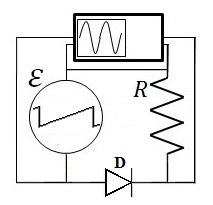
\includegraphics[scale=0.8]{Caracterizar-Diodo}
   \caption{Circuito que consta de una fuente de voltaje que varia en el tiempo de forma lineal, una resistencia R y un diodo D. Conectado a la resistencia y a la fuente se encuentra un osciloscopio}
   \label{fig:Car-Dio}
\end{figure}

Para realizar las mediciones correspondientes, se conectó el osciloscopio en paralelo con la resistencia para medir la corriente circulante y mediante a una \textit{ficha T} se conecto a la fuente para medir el voltaje de entrada, con el fin de utilizar la frecuencia de esa señal como \textit{trigger externo} y, ademas, para medir la caída de potencial en el diodo a partir de la diferencia entre la tension entregada por el generador y la medida sobre la resistencia. Se configuro el generador de funciones para que generara una onda triangular con una frecuencia  $F = (50 \pm 0.005)hz$ y con una amplitud pico-pico de $(16 \pm 0.2)V$, que se dispuso de esa forma para que, en el caso del Zenek, se pudiera apreciar el efecto avalancha, y se configuró el osciloscopio para que midiera sobre medio periodo de la oscilación. De esta forma, el osciloscopio obtenía datos correspondientes a 2500 valores distintos de voltaje distribuidos uniformemente en el intervalo $[-8V;8V]$ que, mediante un programa de adquisición de datos, eran importados a una computadora para su posteriormente análisis. Este proceso fue el mismo para los tres diodos utilizados.

\subsection{Rectificadores de Corriente}
Una vez terminada la caracterización de los diodos, se procedió a construir rectificadores de corriente. Para cada uno de estos, se exploraron los parámetros para ver en que punto se podía obtener una corriente continua.

\subsubsection{Rectificador de media onda}
En primer lugar, se construyó un rectificador de media onda utilizando un generador de funciones como fuente sinusoidal, un diodo simple, una resistencia $R = (5.00 \pm 0.05)k\Omega$ y un capacitor $C = (9.81 \pm 0.07)\mu F$ conectado en paralelo a la resistencia como se ilustra en la \textbf{Figura \ref{fig:Re-M-O}}. De manera análoga al método utilizado para caracterizar lo diodos, se conectó un canal del osciloscopio en paralelo a la resistencia, para medir la corriente circulante; y el otro en paralelo a la fuente. Y, ademas, se aseguró la continuidad de los cables y que esta no se viera comprometida con movimientos aleatorios utilizando el multimetro.

\begin{figure}[H]
\centering
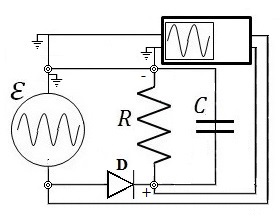
\includegraphics[scale=0.8]{Rectificador-Media-Onda}
   \caption{Circuito sobre el cual se midio el \textit{ripple} de la corriente de salida para distintas frecuencias, consta de un diodo simple D, una resistencia R y una capacitancia C que no fueron modificados durante el experimento. }
   \label{fig:Re-M-O}
\end{figure}

Para medir el ripple de la corriente de salida, se configuró el osciloscopio para que eliminara la componente continua de la señal y midiera la amplitud pico-pico. Fijada una frecuencia en el generador de funciones, se registraba la amplitud marcada por el osciloscopio y se consideró un error para cada medición lo suficientemente grande como para que contuviera las fluctuaciones de ese valor en pantalla además del error instrumental descrito anteriormente. El proceso se iteró con distintas frecuencias.  Ademas, como método alternativo de medicion, se importaron los datos del osciloscopio a la computadora con y sin la componente continua de la señal por medio de un programa de adquisición de datos para un posterior análisis estadístico.

\subsubsection{Rectificador de onda completa}
En este caso se intentó diseñar un rectificador de onda completa, para esto se construyó un circuito que constaba de cuatro diodos simples idénticos, una resistencia variable por décadas y una fuente de voltaje sinusoidal dispuestos como se muestra en la \textbf{Figura \ref{fig:Rect-O}}. Previo a la construcción se observó que los cables no tuvieran discontinuidades. Cabe aclarar que durante esta experiencia no se utilizó el generador de funciones como fuente ya que, como los canales de salida del mismo tenían descarga a tierra, al igual que los del osciloscopio, seria necesario conectarlos a una misma terminal, pero como se puede ver en la \textbf{Figura \ref{fig:Rect-O}} eso no era posible, por lo cual se utilizó una fuente flotante. 

\begin{figure}[H]
\centering
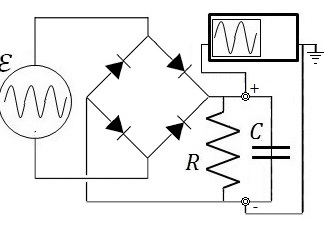
\includegraphics[scale=0.8]{Rectificador-Onda-Completa}
   \caption{Circuito que consta de una fuente de voltaje que varia en el tiempo de forma lineal, una resistencia R y un diodo D. Conectado a la resistencia y a la fuente se encuentra un osciloscopio}
   \label{fig:Rect-O}
\end{figure}

Al no disponer de una fuente de frecuencia variable, debió variarse la resistencia, la cual es proporcional al tiempo de carga del capacitor. Esto permite reducir la carga que un capacitor adquiere en un período de la señal y, por lo tanto, es equivalente a aumentar la frecuencia. 

Para medir el ripple de la corriente de salida se realizó el mismo proceso que para el rectificador de media onda, pero no se utilizó el método alternativo. Cabe destacar, que durante las mediciones se pudo observar que los movimientos del aire producidos por un ventilador de la sala e incluso ruidos cercanos provocaban un efecto microfonico que interfería con las mediciones, por lo cual se intento mantener silencio en ese momento y se evitó medir en los momentos con viento.


%%%%%%%%%%%%%%%%%%%%%%%%%%%%%%%%%%%%%%%%%%%%%%%%%%%%%%%%%%%%%%%%%%%%%%%%%%%%%%%%%%%%%%%%%%%%%%%%%%%%%%%%%%%%%%%%%%%%%%%%%%%%%%%%
% 4.DISCUSIÓN Y RESULTADOS: todo lo que se obtuvo y explicación. Graficos, tablas.
%%%%%%%%%%%%%%%%%%%%%%%%%%%%%%%%%%%%%%%%%%%%%%%%%%%%%%%%%%%%%%%%%%%%%%%%%%%%%%%%%%%%%%%%%%%%%%%%%%%%%%%%%%%%%%%%%%%%%%%%%%%%%%%%

\section{Resultados}
\label{sec:discusion}

\subsection{Caracterización de Instrumentos}

A la hora de caracterizar los instrumentos, como se dijo, se relevaron las curvas $V_f(t)$ y $V_R(t)$. Usando las leyes de Kirchoff, se obtuvo la caida de potencial en el diodo $V_D(t) = V_e(t)-V_R(t)$ y la corriente $I(t) = \frac{V_R(t)}{R}$ con $R = (600 \pm 6)\Omega$. Para el diodo simple, la relación entre $V_D$ e $I$ puede verse en la \textbf{Figura \ref{fig:simple_feo}}.

\begin{figure}[H]
\centering
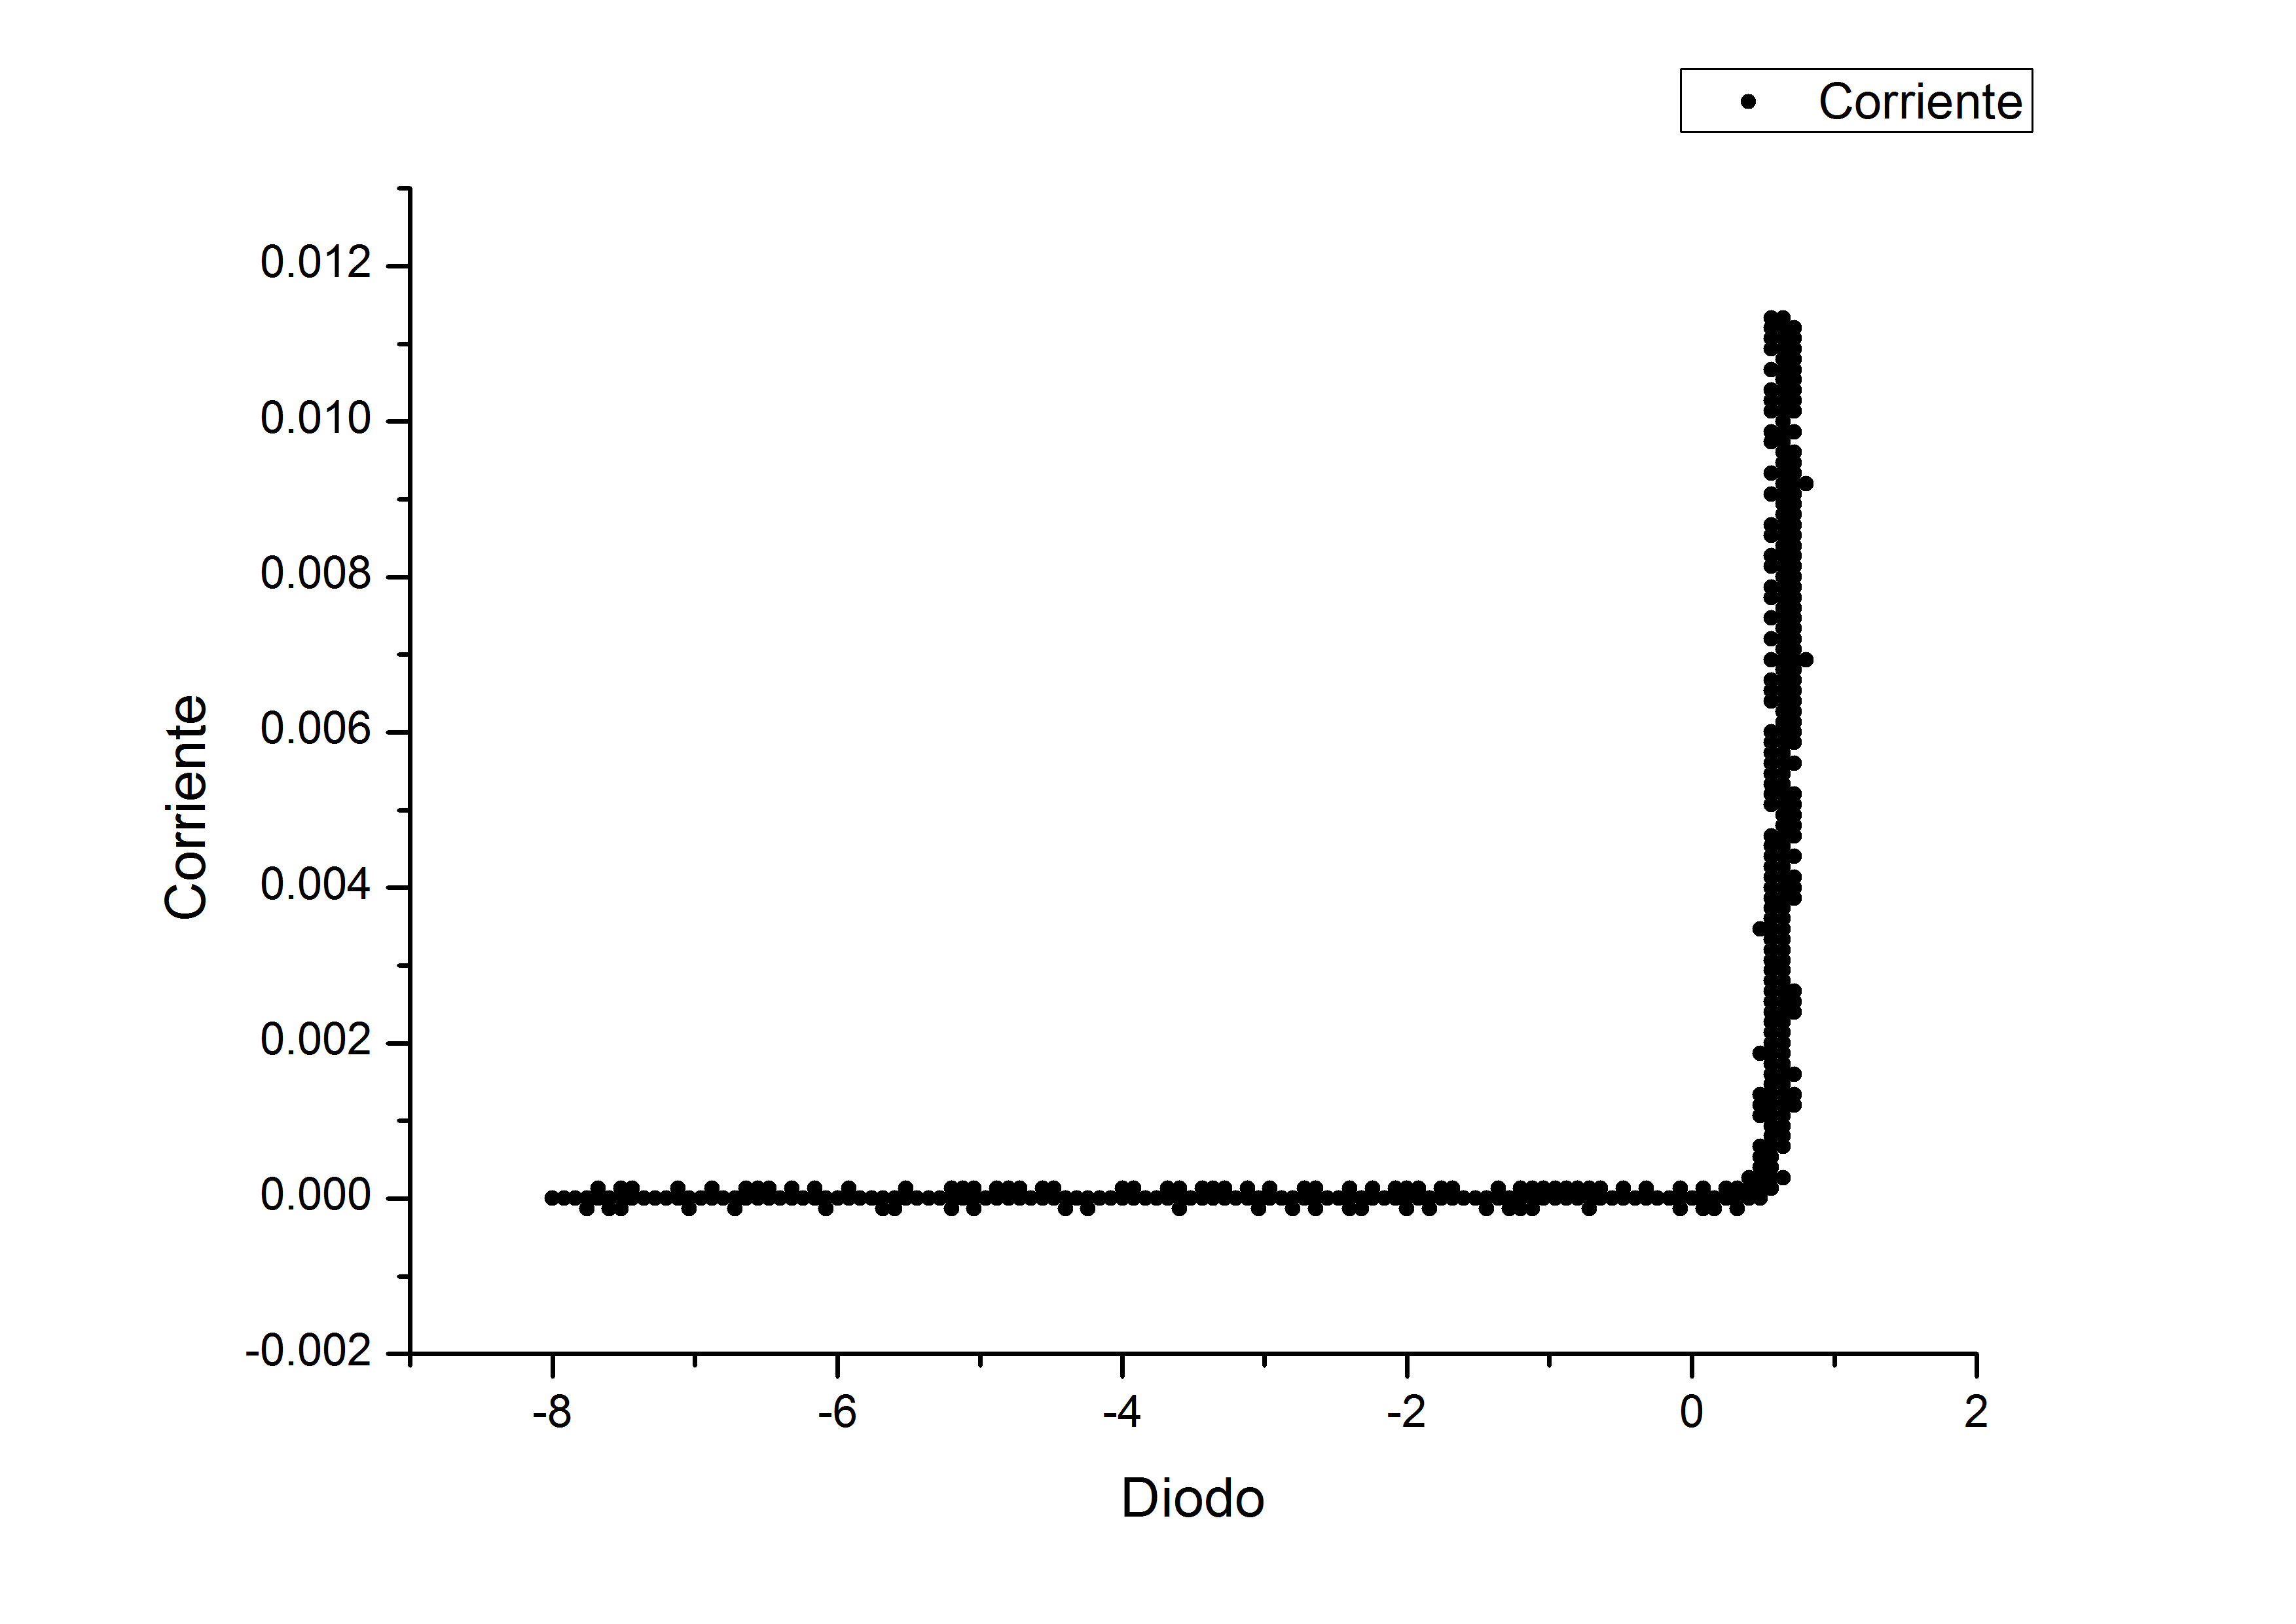
\includegraphics[scale=0.36]{simple_feo}
   \caption{Grafico inicial con la relacion entre $V_D$ e $I$ para un diodo simple obtenida indirectamente donde puede verse la gran dispersión de la curva}
   \label{fig:simple_feo}
\end{figure}

Claramente, la curva de la \textbf{Figura \ref{fig:simple_feo}} posee una enorme cantidad de puntos muy cercanos al punto de resultar indistinguibles. Debido a esto, se buscó suavizar la señal con menos puntos con un método simple. Primero, se configuró un parametro de tolerancia $CT$ como error y se promediaron los valores de todas las corrientes $I(V_D)$ cuyos $V_D$ fueran indistinguibles dentro de este error $CT$. Estos $CT$ se tomaron de forma tal que la cantidad de puntos fuera menor que el que permitiría el error relativo del 3\% que dispone el instrumento aplicado sobre el valor máximo voltaje (en módulo) en cada tira de valores $V_D$. De esta forma, multiples puntos con $V_D$ cercanos fueron condensados en un único punto, permitiendo que la curva sea más clara como puede verse en la \textbf{Figura \ref{fig:simple_mejor}}. Un ajuste lineal de $R-Square = 0.97052$ asegura la bondad del ajuste con una pendiente $m_s = (0.02557 \pm 0,0018)\Omega^{-1}$ tal que a través de \eqref{Aprox} resulta $\frac{1}{m_s} = (39 \pm 3)\Omega= R_s$ la resistencia del diodo simple.

\begin{figure}[H]
\centering
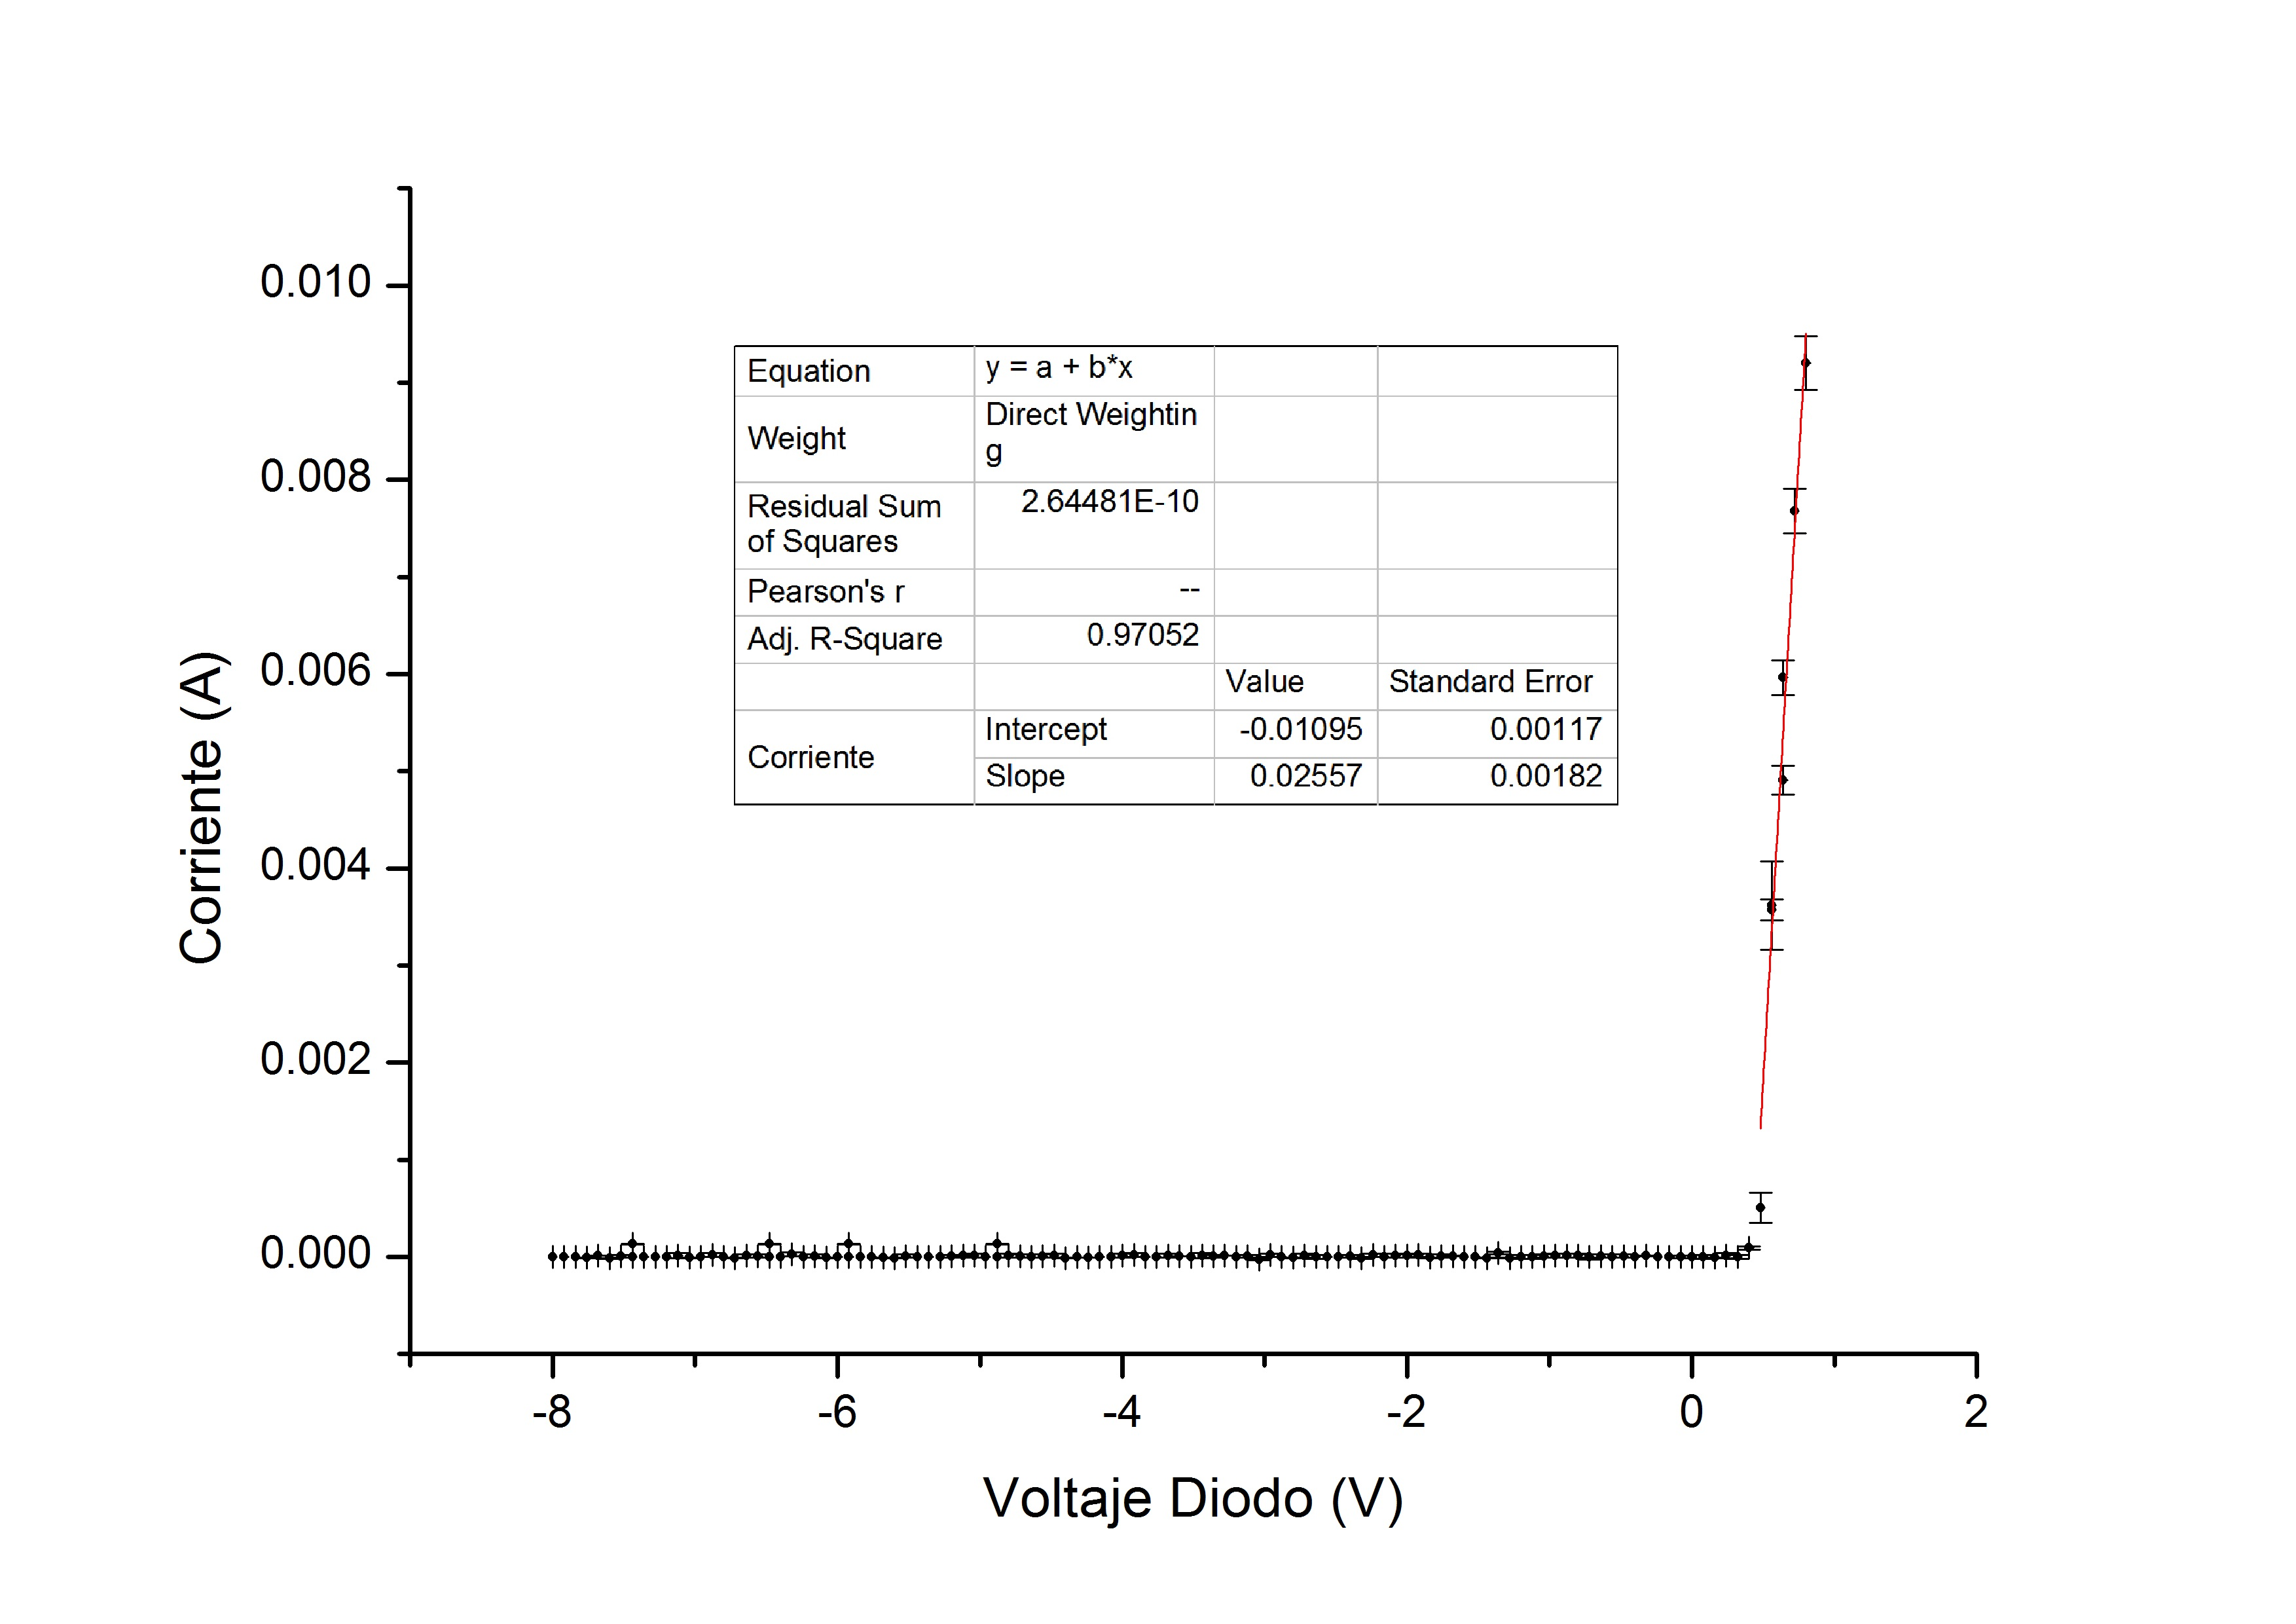
\includegraphics[scale=0.36]{simple_mejor}
   \caption{Grafico con la relacion entre $V_D$ e $I$ tras aplicar un análisis más fino para un diodo simple. El ajuste lineal en los últimos puntos asegura la linealidad del diodo para altos voltajes.}
   \label{fig:simple_mejor}
\end{figure}

El proceso anterior debió aplicarse también a los resultados obtenidos para el diodo Zenek y el diodo LED. En el caso particular del Zenek, la tolerancia se tomó como $CT = 3.2E-6$ y en base al resultado fue posible apreciar el \textit{efecto avalancha} como puede verse en la \textbf{Figura \ref{fig:zenek}}. 

\begin{figure}[H]
\centering
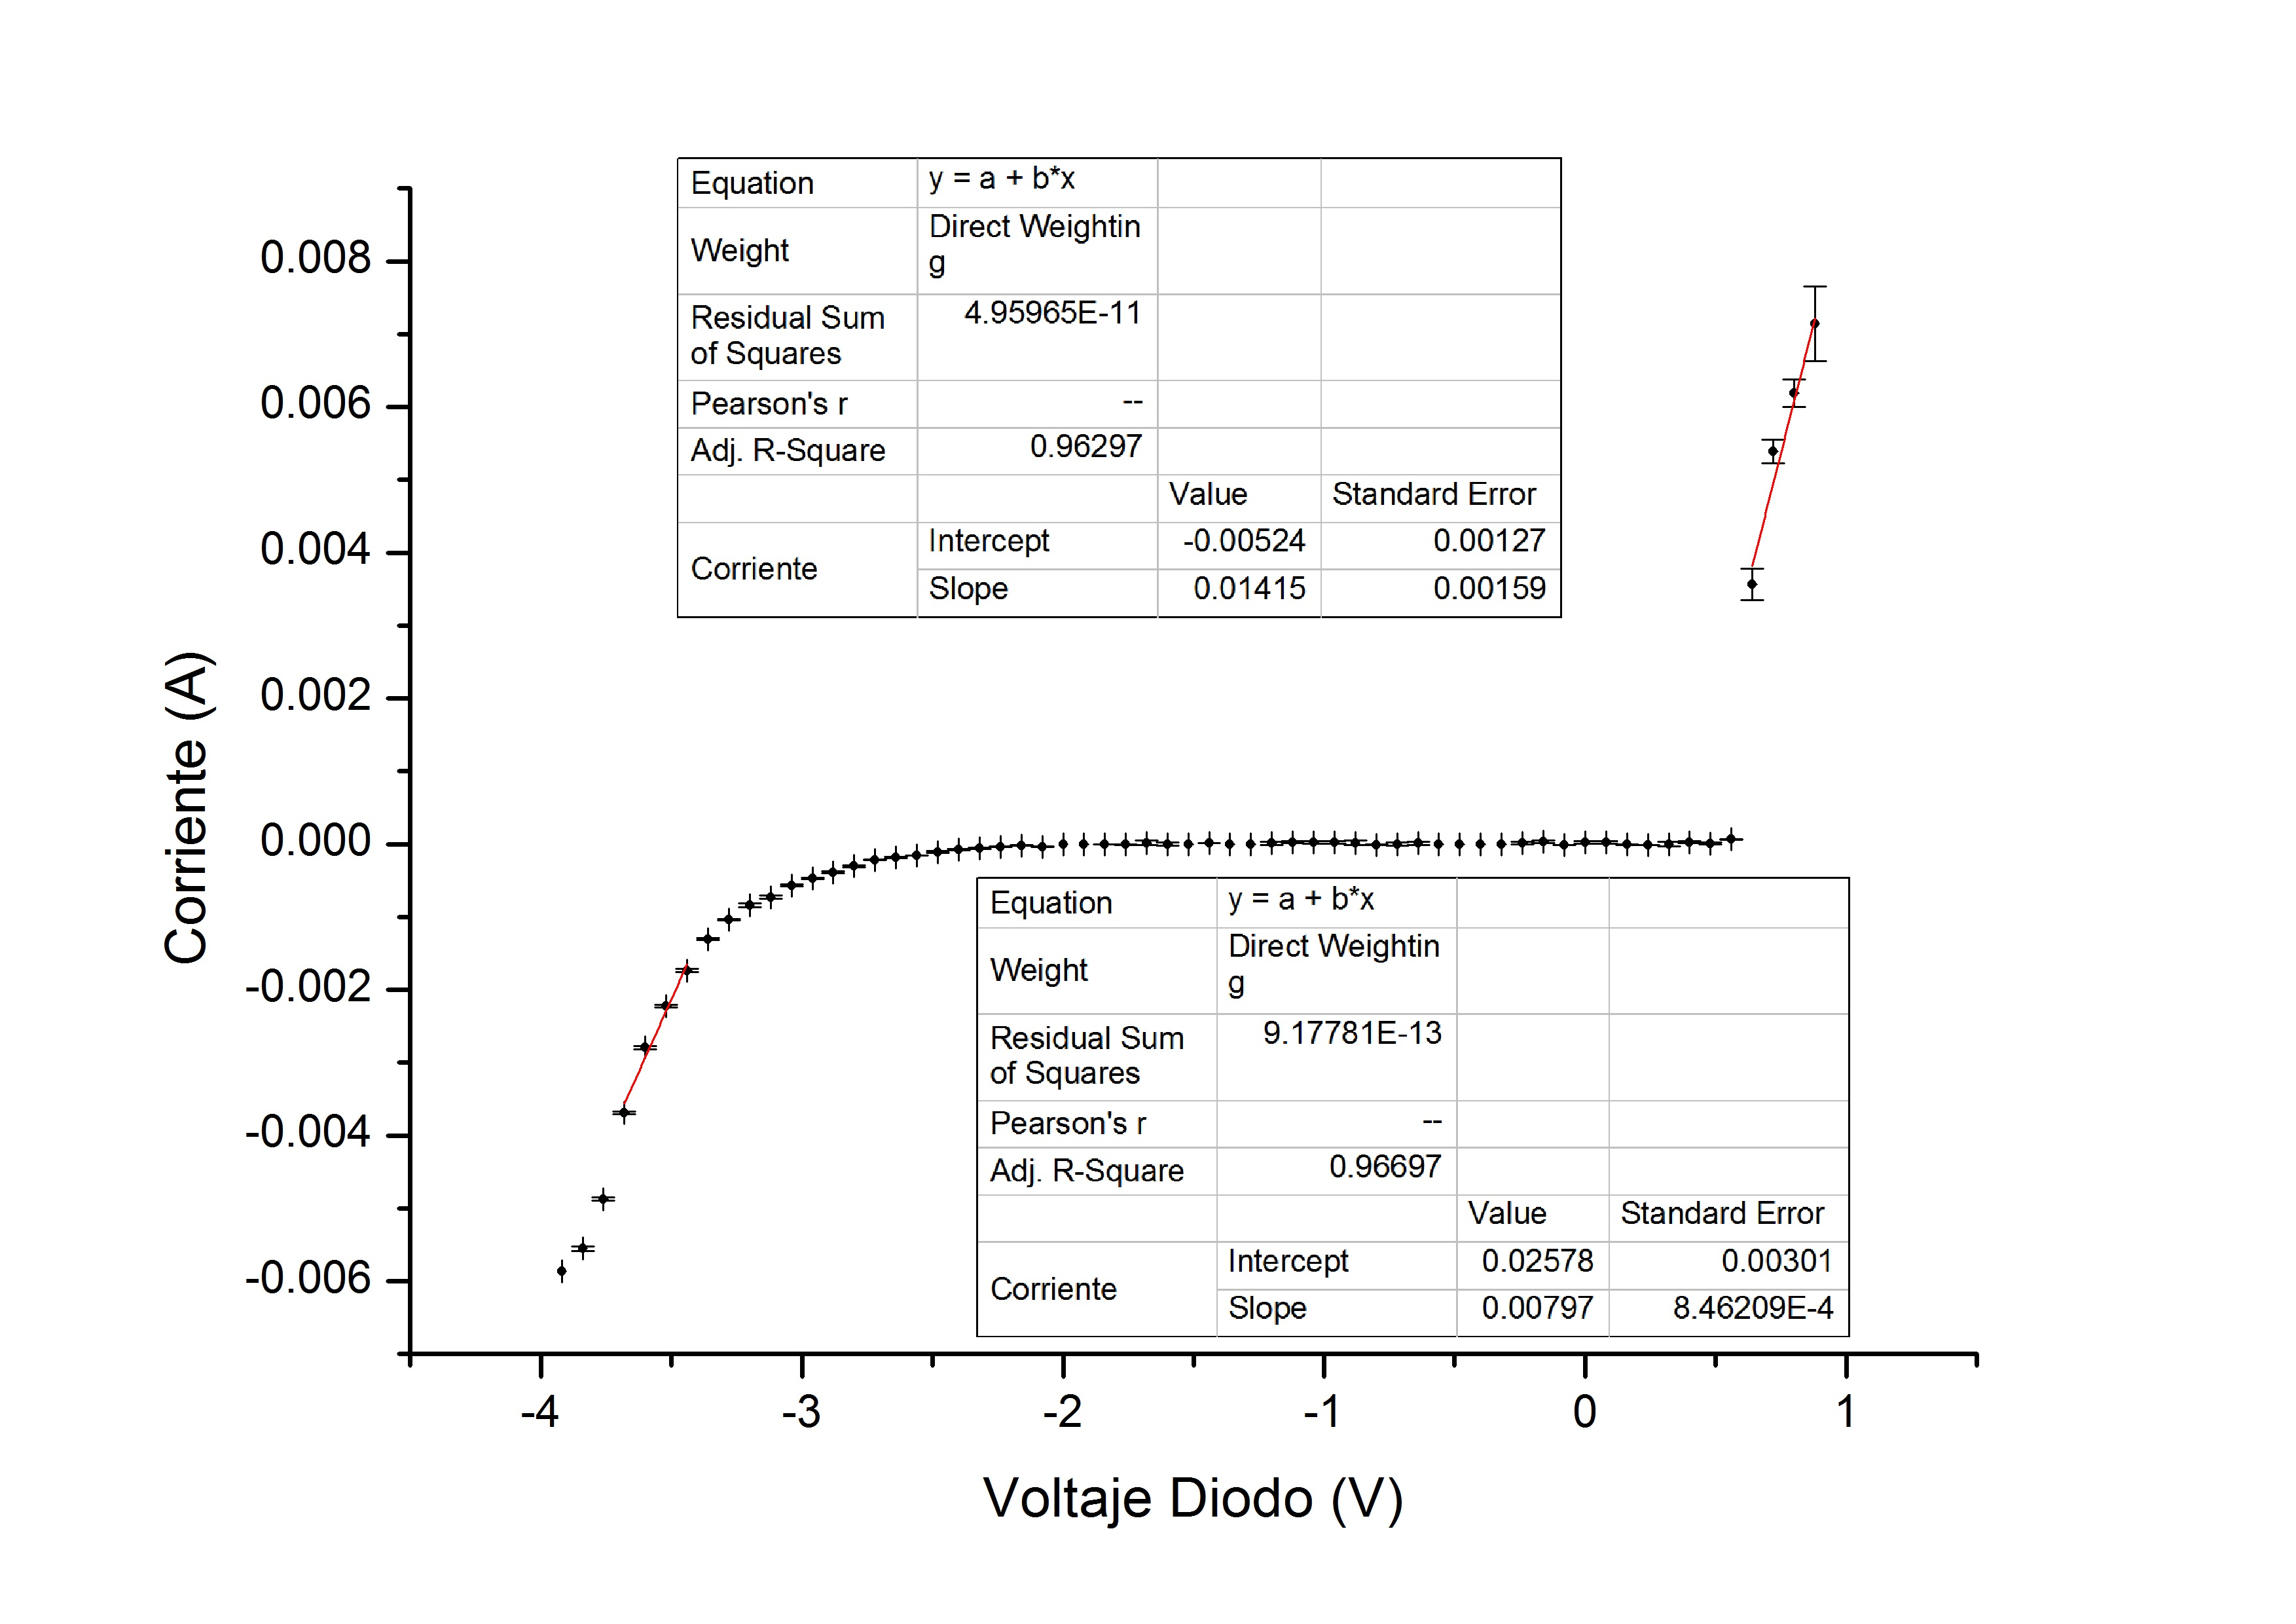
\includegraphics[scale=0.36]{zenek}
   \caption{Grafico con la relacion entre $V_D$ e $I$ para un diodo Zenek tras aplicar un análisis más fino. Los ajustes lineales en los últimos puntos y en los primeros puntos aseguran la linealidad del diodo a partir de determinados voltajes.}
   \label{fig:zenek}
\end{figure}

El ajuste de los primeros puntos referentes al \textit{efecto avalancha} arroja un $R-Square = 0.96697$ que asegura la bondad del ajuste con una pendiente $m_I^{(z)} = (0.0080 \pm 0.0008)\Omega^{-1}$ tal que la resistencia del diodo a resulta $R_I^{(z)} = (125 \pm 13)\Omega$. Para los puntos finales, el ajuste arroja un $R-Square = 0.96297$ con una pendiente $m_D^{(z)} = (0.0142 \pm 0.0016)\Omega^{-1}$ tal que la resistencia para corriente en directa resulta según \eqref{Aprox} $R_D^{(z)} = (70 \pm 8)\Omega$.

Finalmente, para el caso del diodo LED la tolerancia se tomó como $CT = 6.4E-7$, arrojando el gráfico de la \textbf{Figura \ref{fig:LED}}. El ajuste lineal de los ultimos puntos arroja un $R_Square = 0.93178$ con una pendiente $m_L = (0.023 \pm 0.003)$ que resulta en una resistencia para corriente directa $R_L = (43 \pm 6)$ siguiendo \eqref{Aprox}.

\begin{figure}[H]
\centering
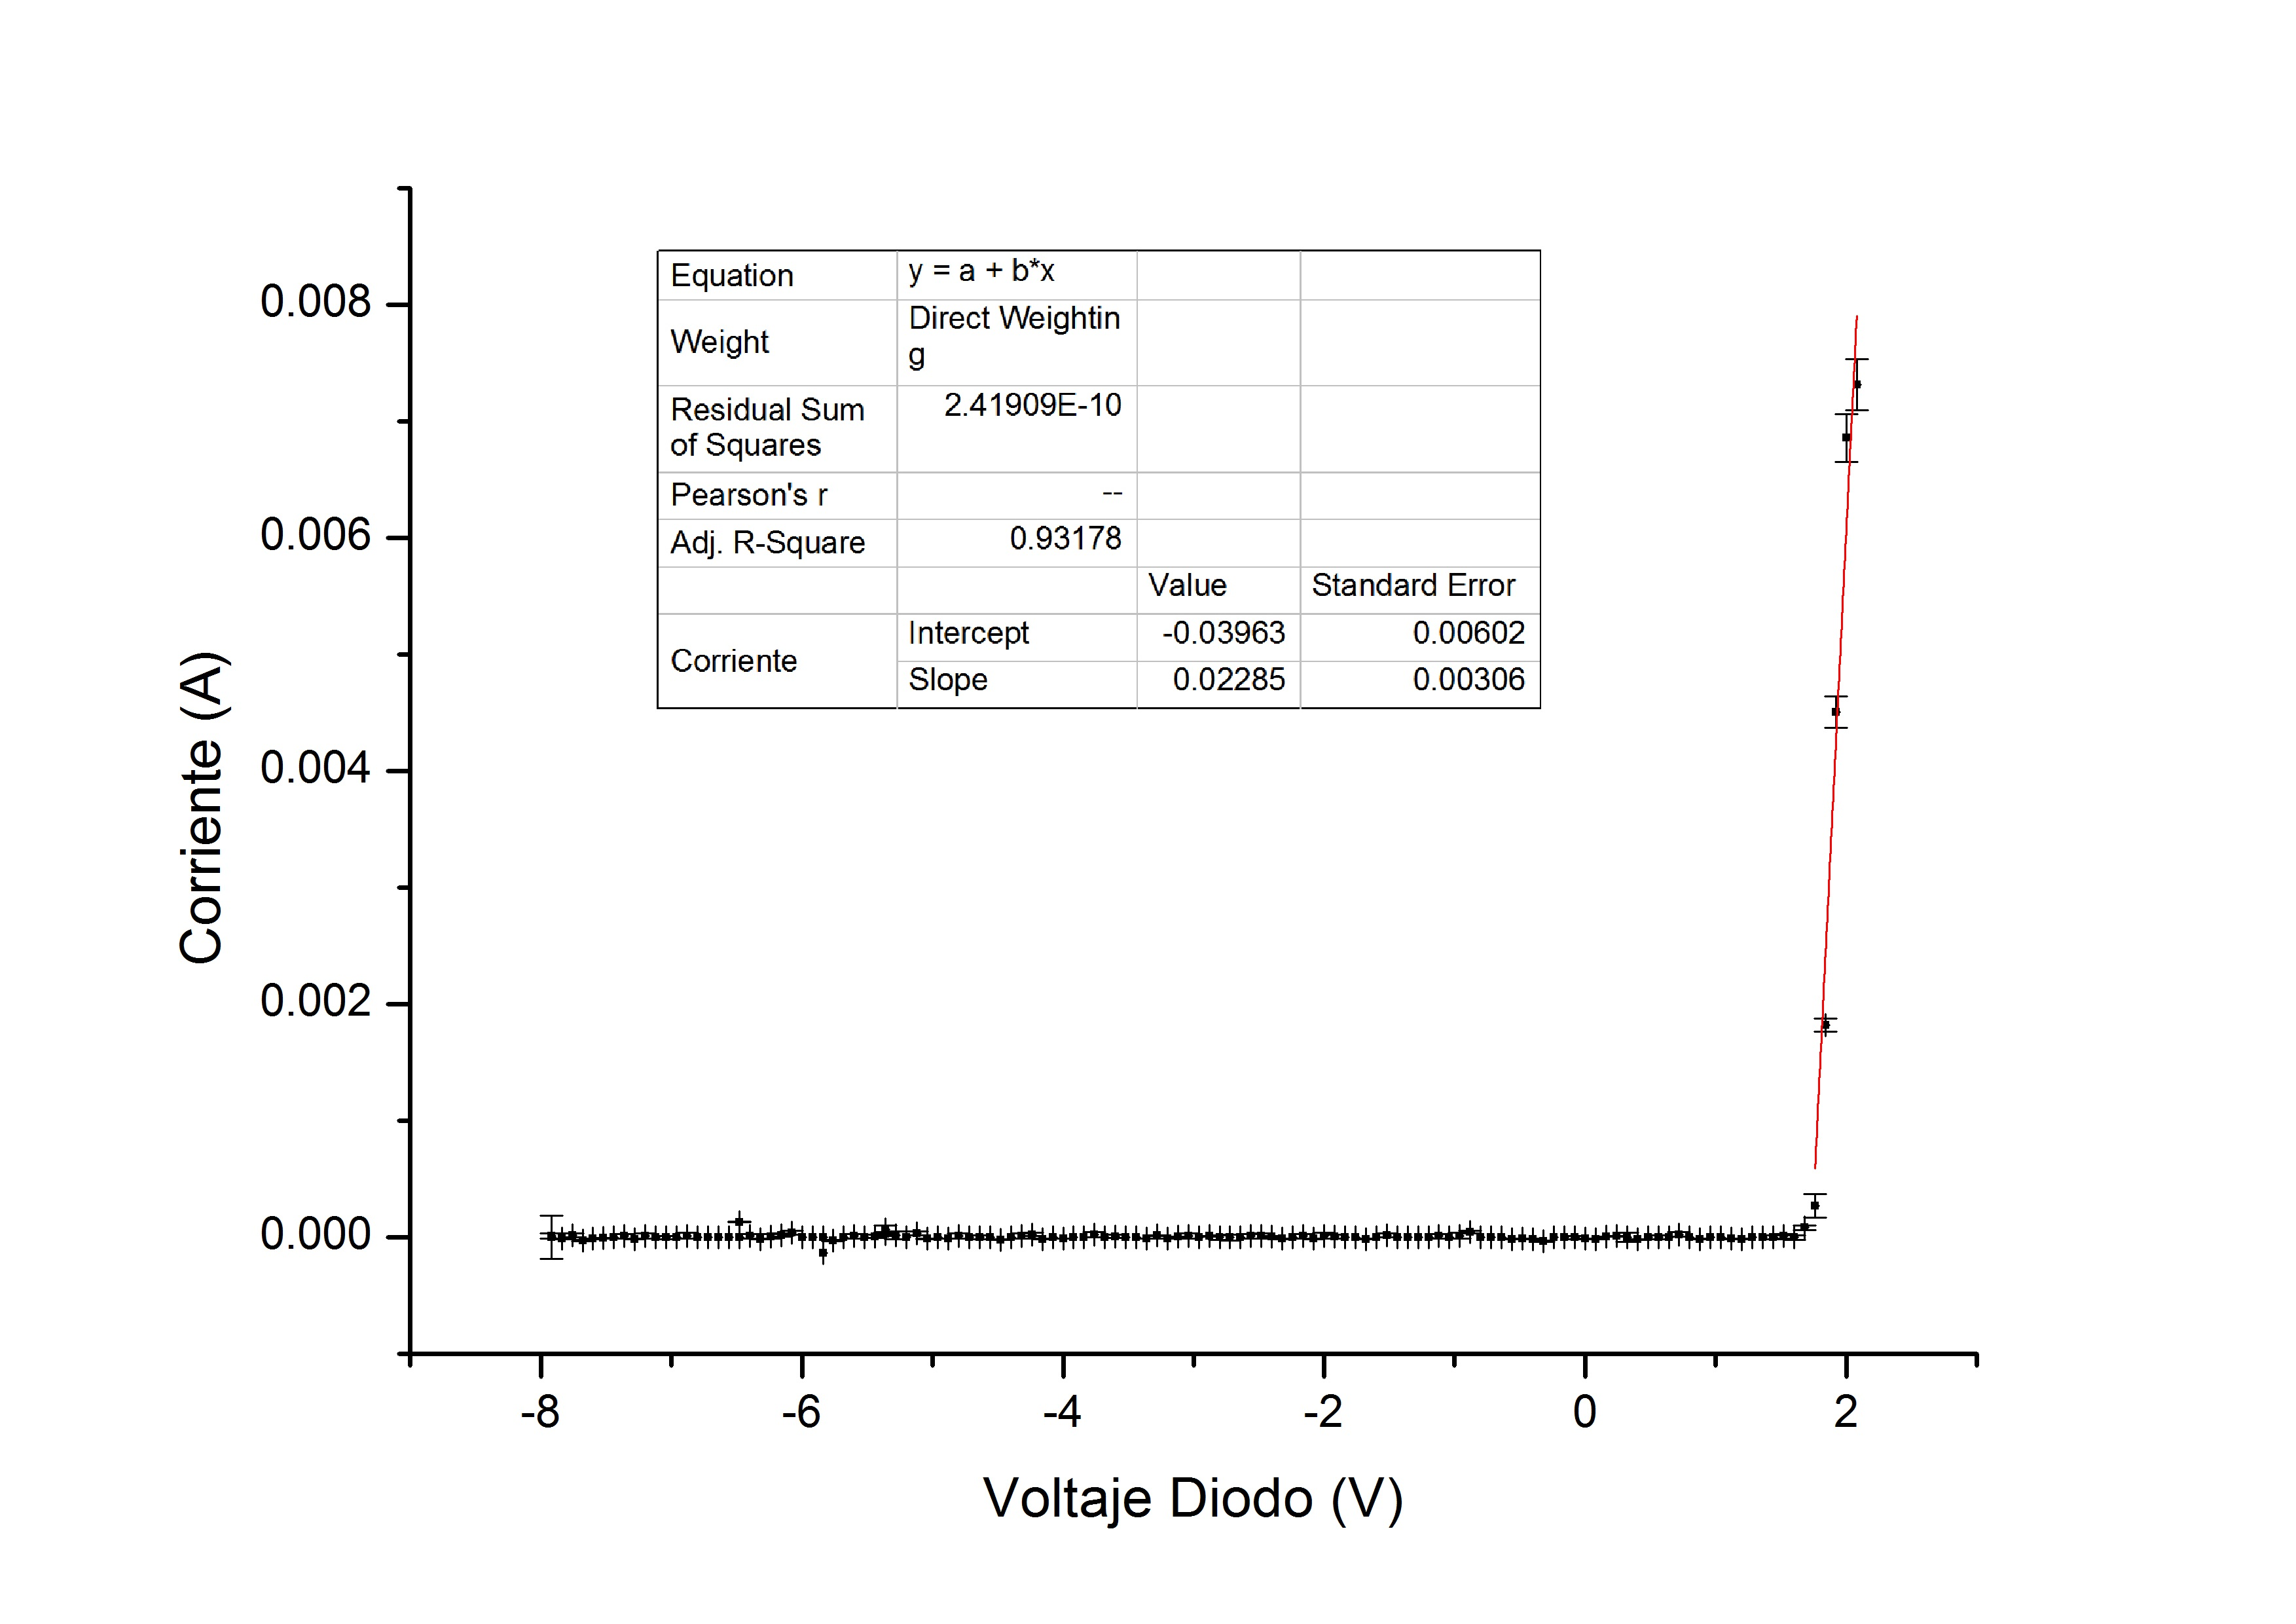
\includegraphics[scale=0.36]{LED}
   \caption{Grafico con la relacion entre $V_D$ e $I$ para un diodo LED tras aplicar un análisis más fino. El ajuste lineal en los últimos puntos permite asumir un comportamiento lineal para altos voltajes.}
   \label{fig:LED}
\end{figure}



\subsection{Rectificadores de Corriente}



\subsubsection{Rectificador de media onda}

Para cada frecuencia utilizada, se importaron ambas curvas como se dijo previamente. Algunos de los graficos obtenidos sin despreciar la componente continua pueden verse en la \textbf{Figura \ref{fig:rectificaciones}}, donde pueden verse los dos casos extremos de rectificación y un caso intermedio. Como puede verse, a medida que las frecuencias crecían, el ripple disminuía pero la componente continua se mantenía constante, por lo que las mediciones de los picos en este tipo de graficos acarrearían un enorme error. 

\begin{figure}[h]
\begin{subfigure}{0.33\textwidth}
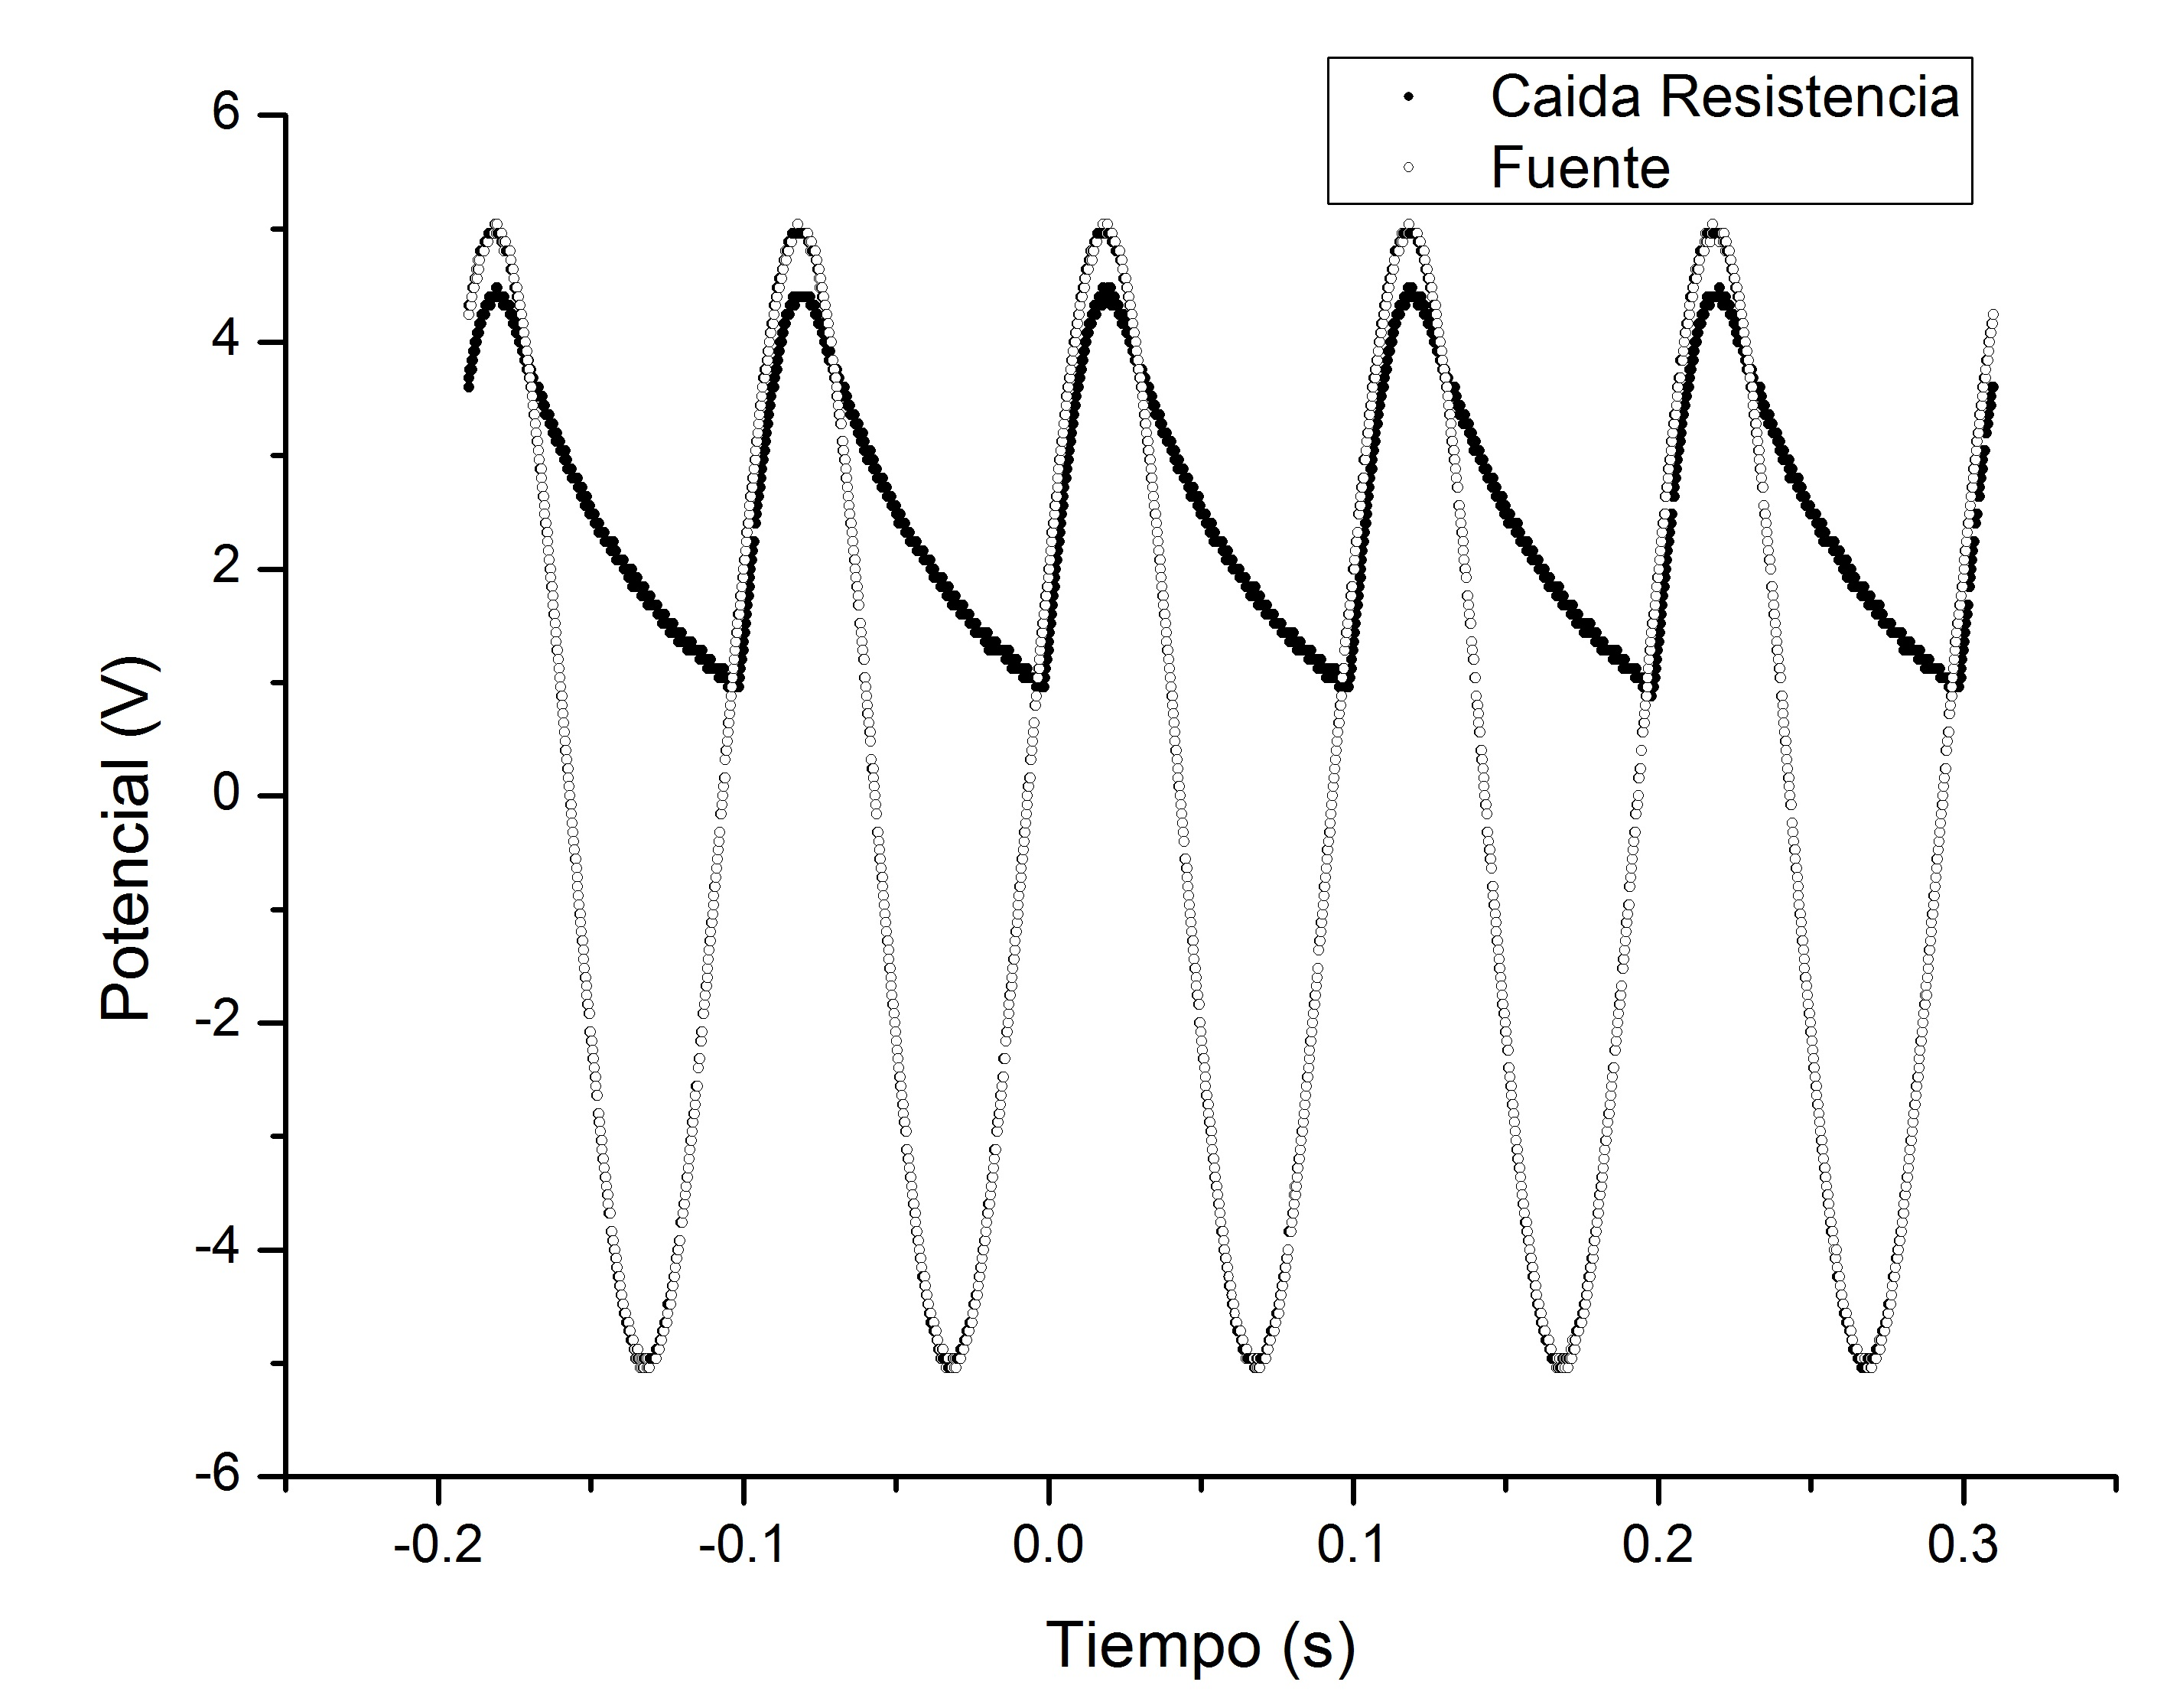
\includegraphics[scale=0.23]{Rectificacion_10hz}
  \caption{Frecuencia de $(10.000\pm0.001)Hz$}
  \label{subfig:rec_10}
\end{subfigure}
\begin{subfigure}{0.33\textwidth}
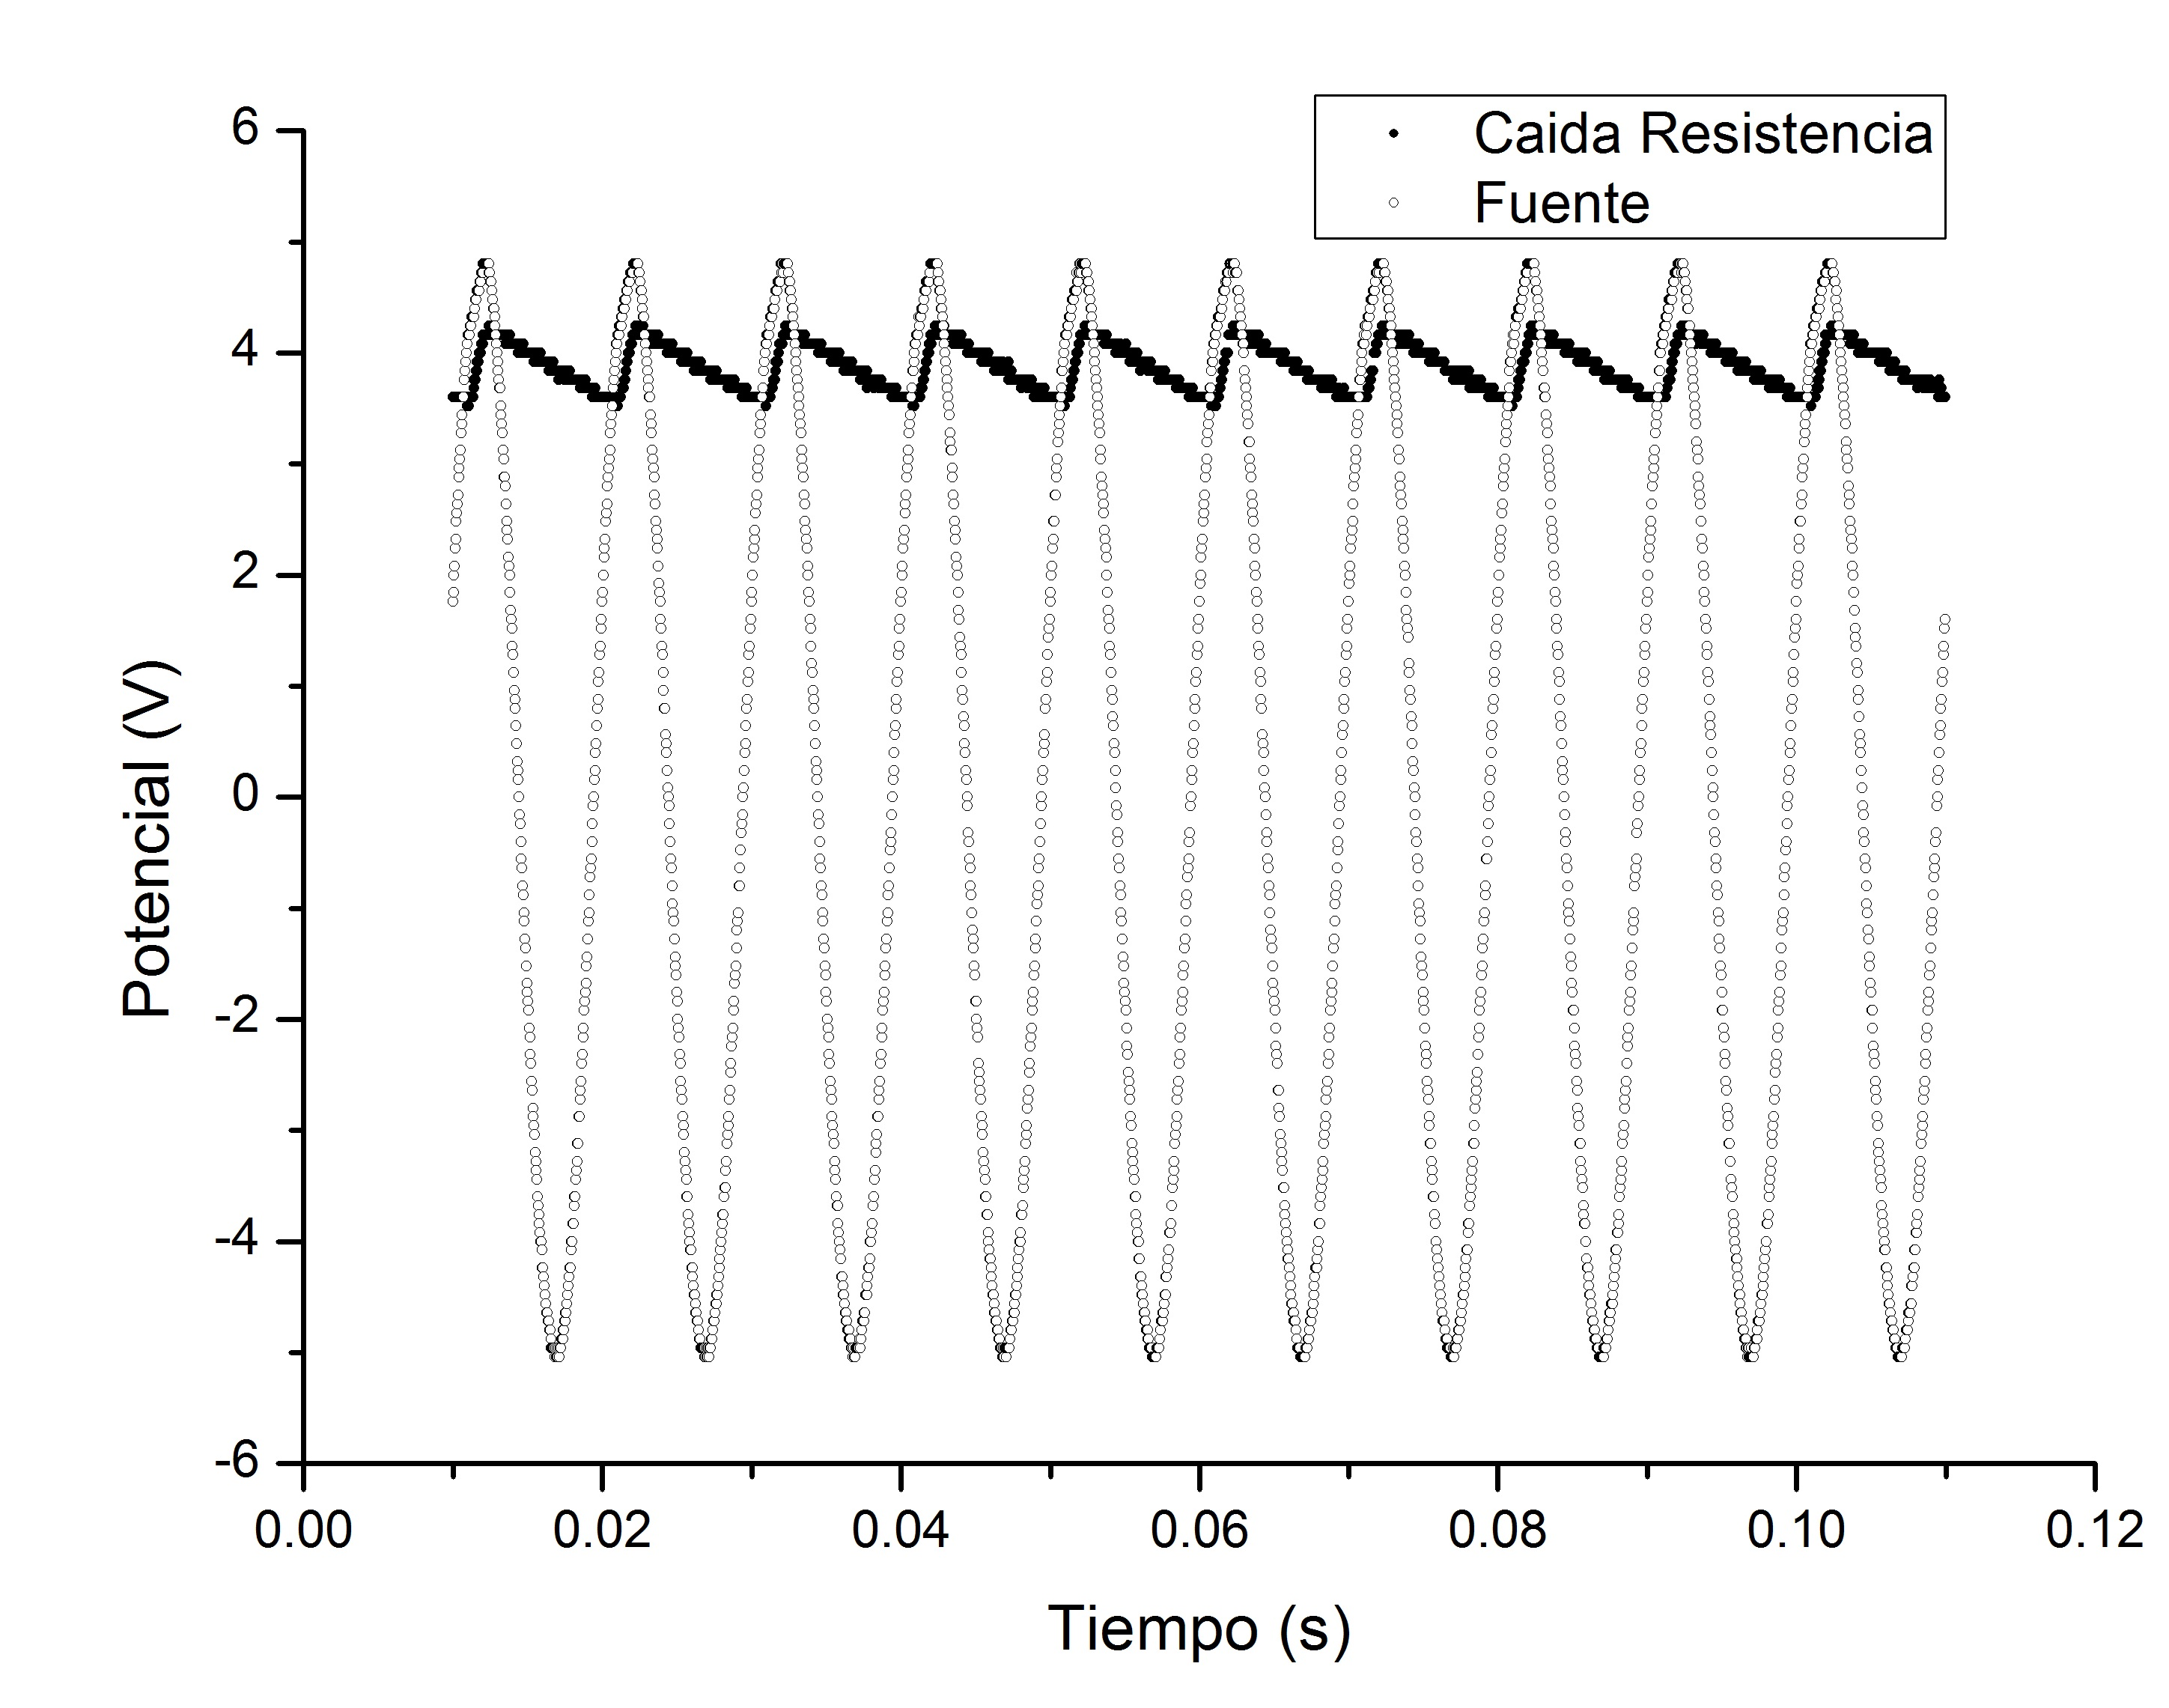
\includegraphics[scale=0.23]{Rectificacion_100hz}
  \caption{Frecuencia de $(100.00\pm0.01)Hz$}
  \label{subfig:rec_100}
\end{subfigure}
\begin{subfigure}{0.33\textwidth}
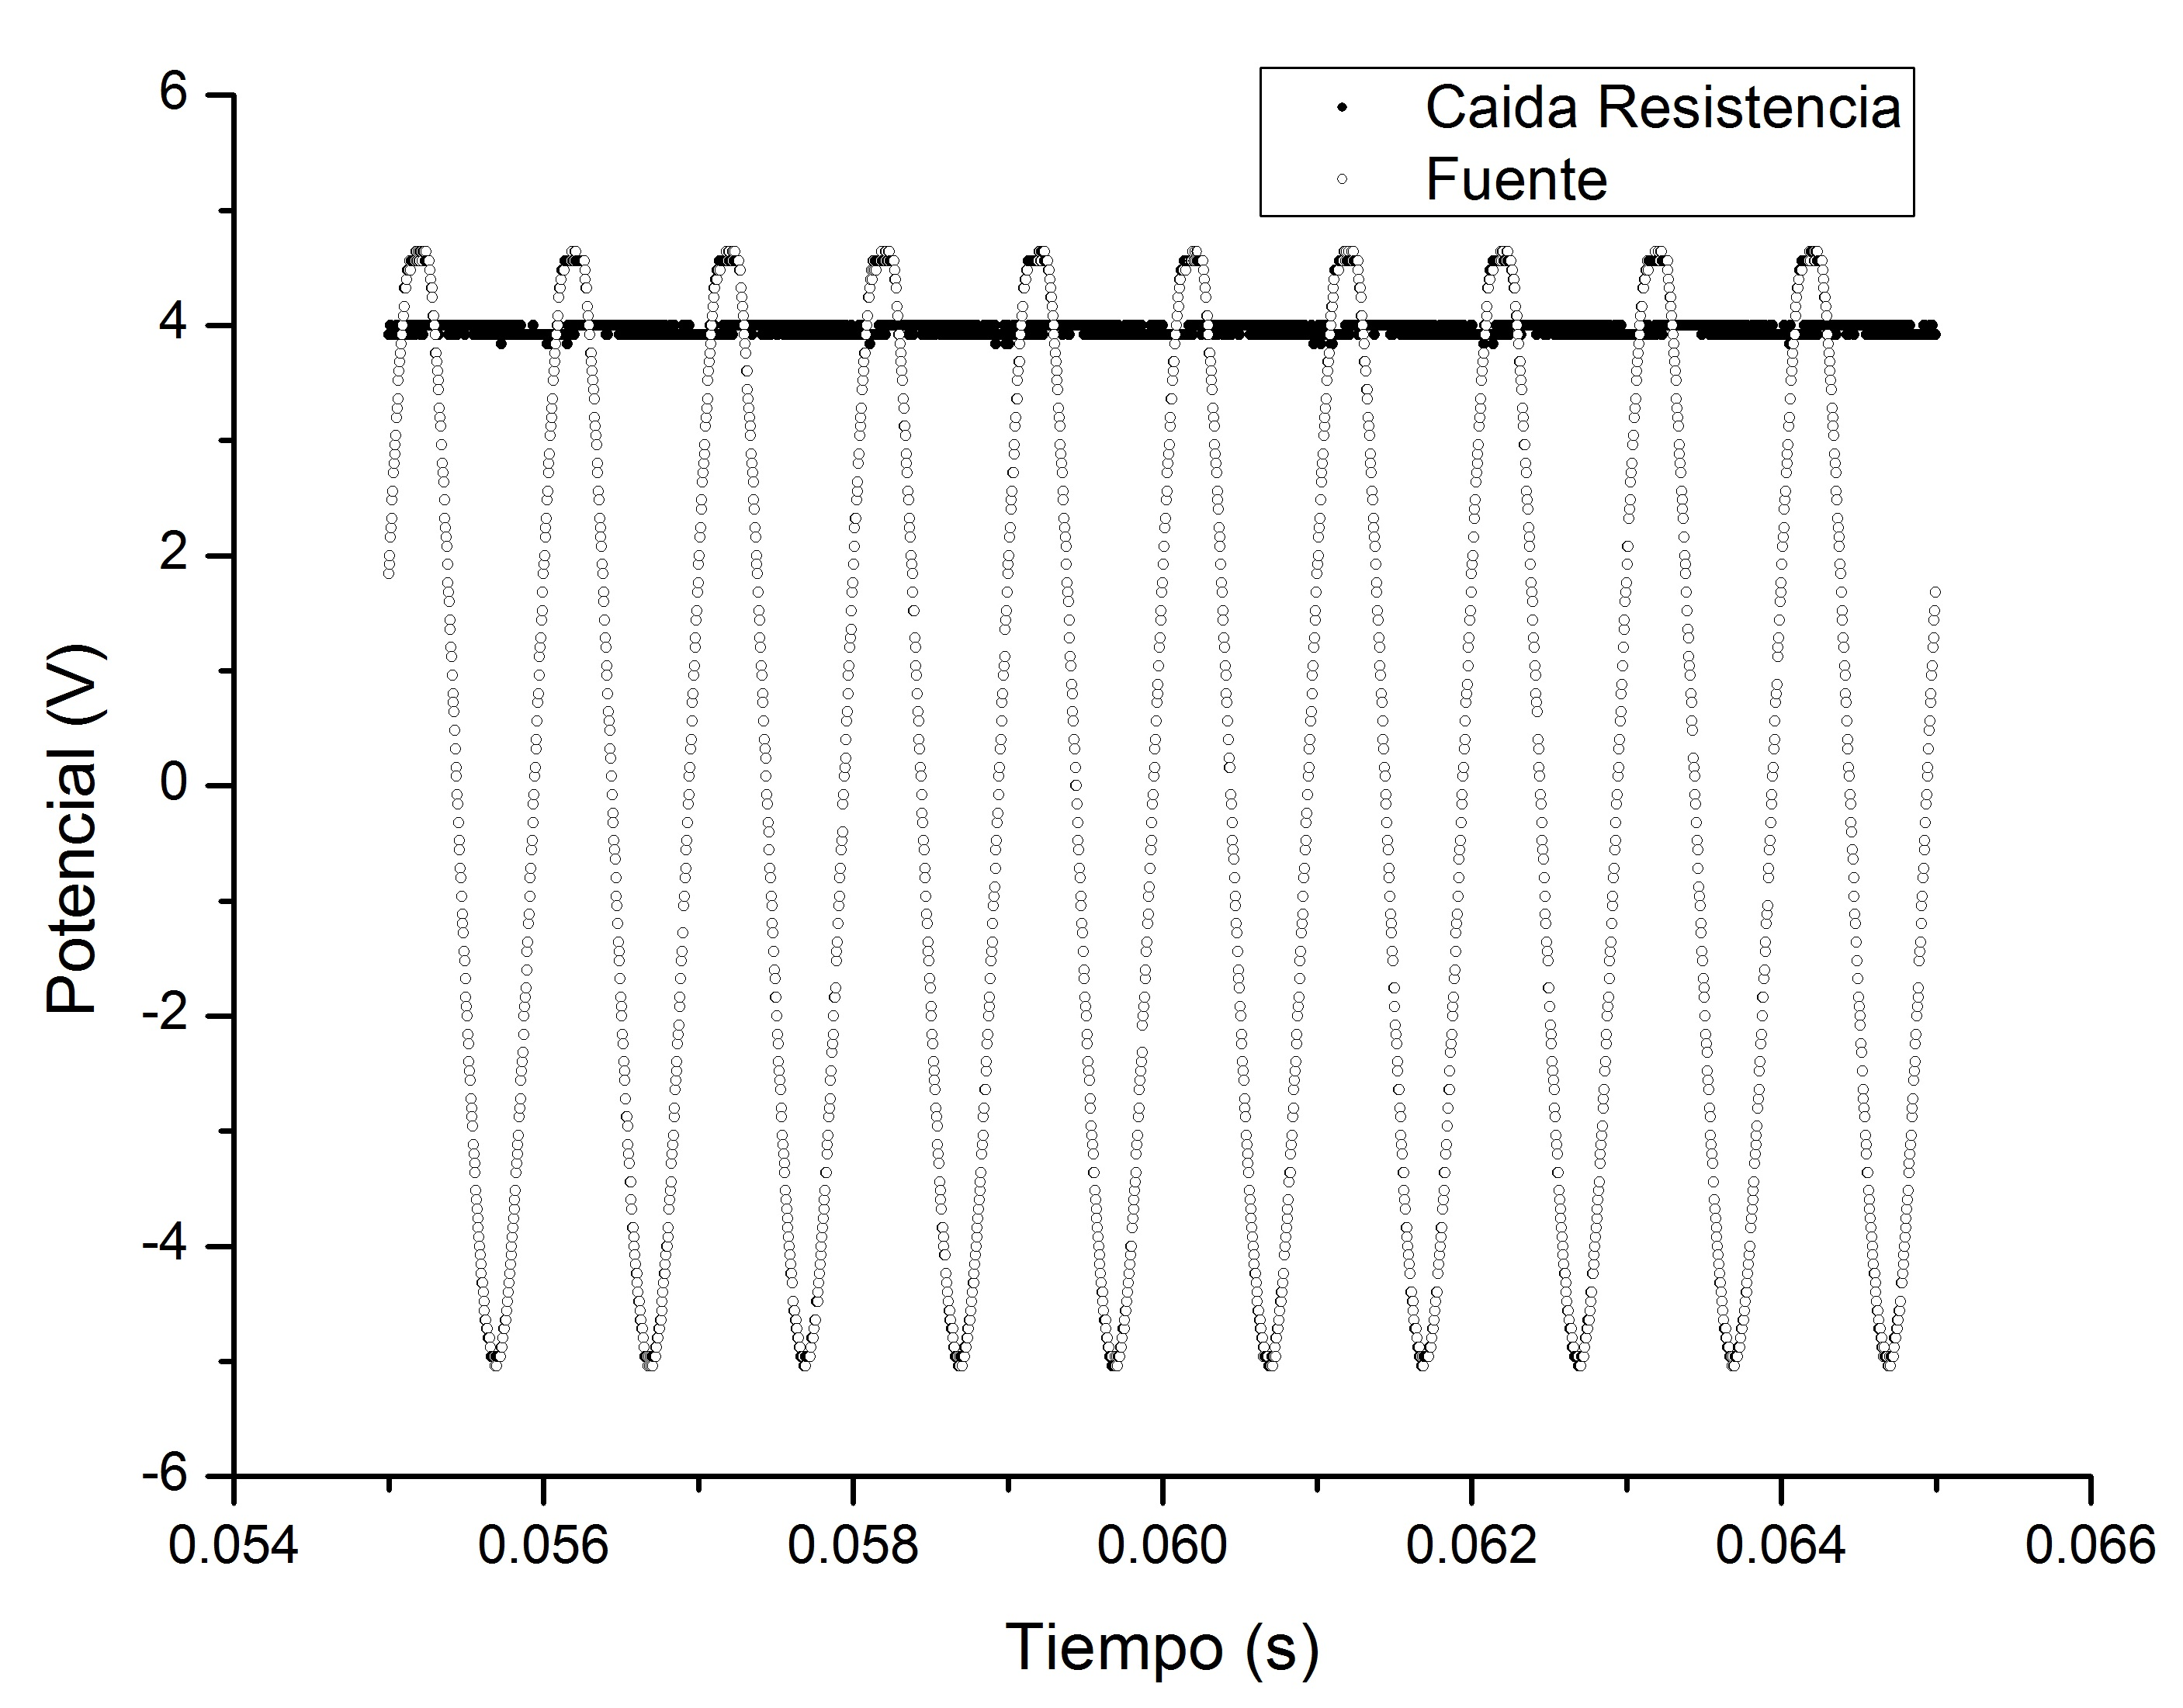
\includegraphics[scale=0.23]{Rectificacion_1000hz}
  \caption{Frecuencia de $(1000.0\pm0.1)Hz$}
  \label{subfig:rec_1000}
\end{subfigure}
  \caption{Voltaje de entrada y de salida para tres frecuencias características que representan los casos extremos e intermedio de la rectificación de señales. }
  \label{fig:rectificaciones}
\end{figure}

\newpage
Por eso, se decidió utilizar los datos cuya componente continua había sido eliminada para hacer un análisis de los picos y así obtener un promedio de máximos y otro de mínimos que, restándose, permitían obtener el ripple para esa frecuencia. Estos valores junto con los proporcionados directamente por el osciloscopio pueden verse en la \textbf{Figura \ref{fig:ripples_media}}, donde claramente puede verse que la mayor parte de los puntos resultan indistinguibles, pues coinciden dentro del error. Esto es realmente así para todos los valores con excepción de los ripples para $F = (50,000 \pm 0,005)Hz$, donde el ripple obtenido a través del osciloscopio es el doble que el obtenido restando los picos. 

\begin{figure}[H]
\centering
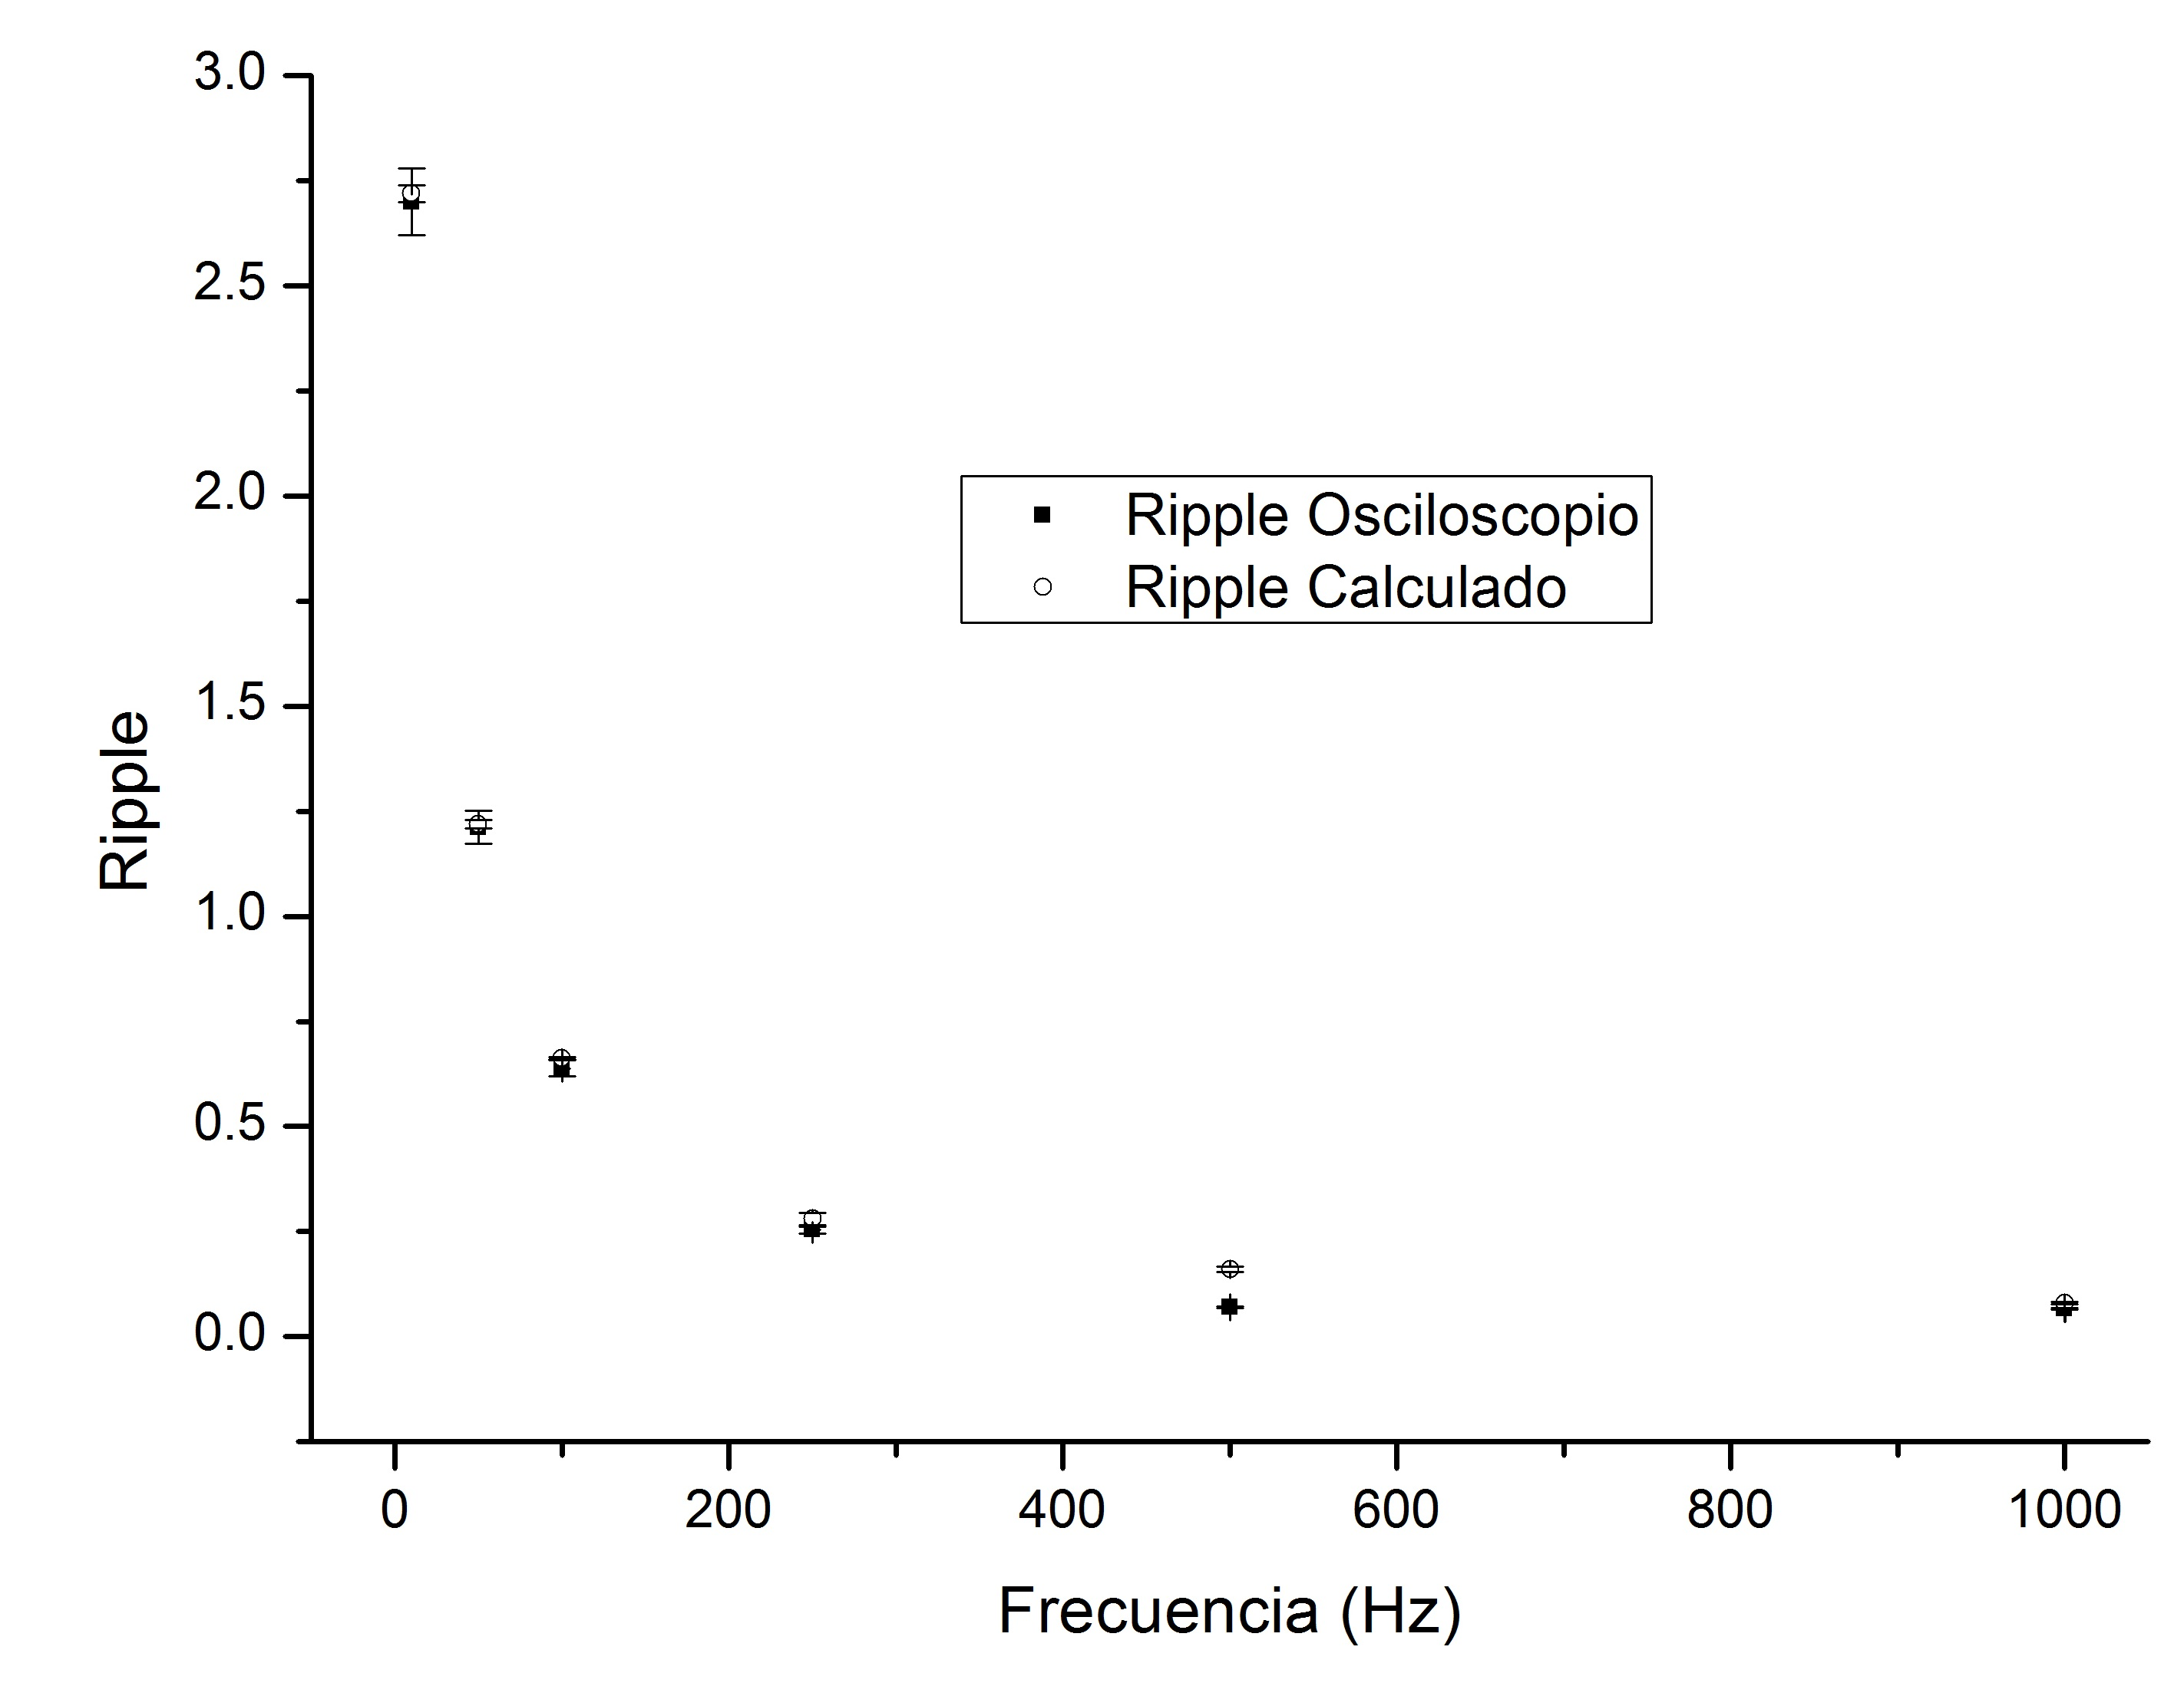
\includegraphics[scale=0.35]{ripples_media}
   \caption{Relación de los ripples medidos directamente del osciloscopio y los calculados restando picos. Puede verse una superposición dentro del error de la mayor parte de los puntos}
   \label{fig:ripples_media}
\end{figure}

Sin embargo, como se dijo, lo que importa es la relación entre el período $T = F^{-1}$ de la señal y el período $\tau = RC = (49.1 \pm 0.8)ms$, por lo que si graficamos las relaciones anteriores en función de $\frac{T}{\tau}$ en lugar de $F$, obtenemos los graficos de la \textbf{Figura \ref{fig:ripples_Tau}}.

\begin{figure}[h]
\begin{subfigure}{0.5\textwidth}
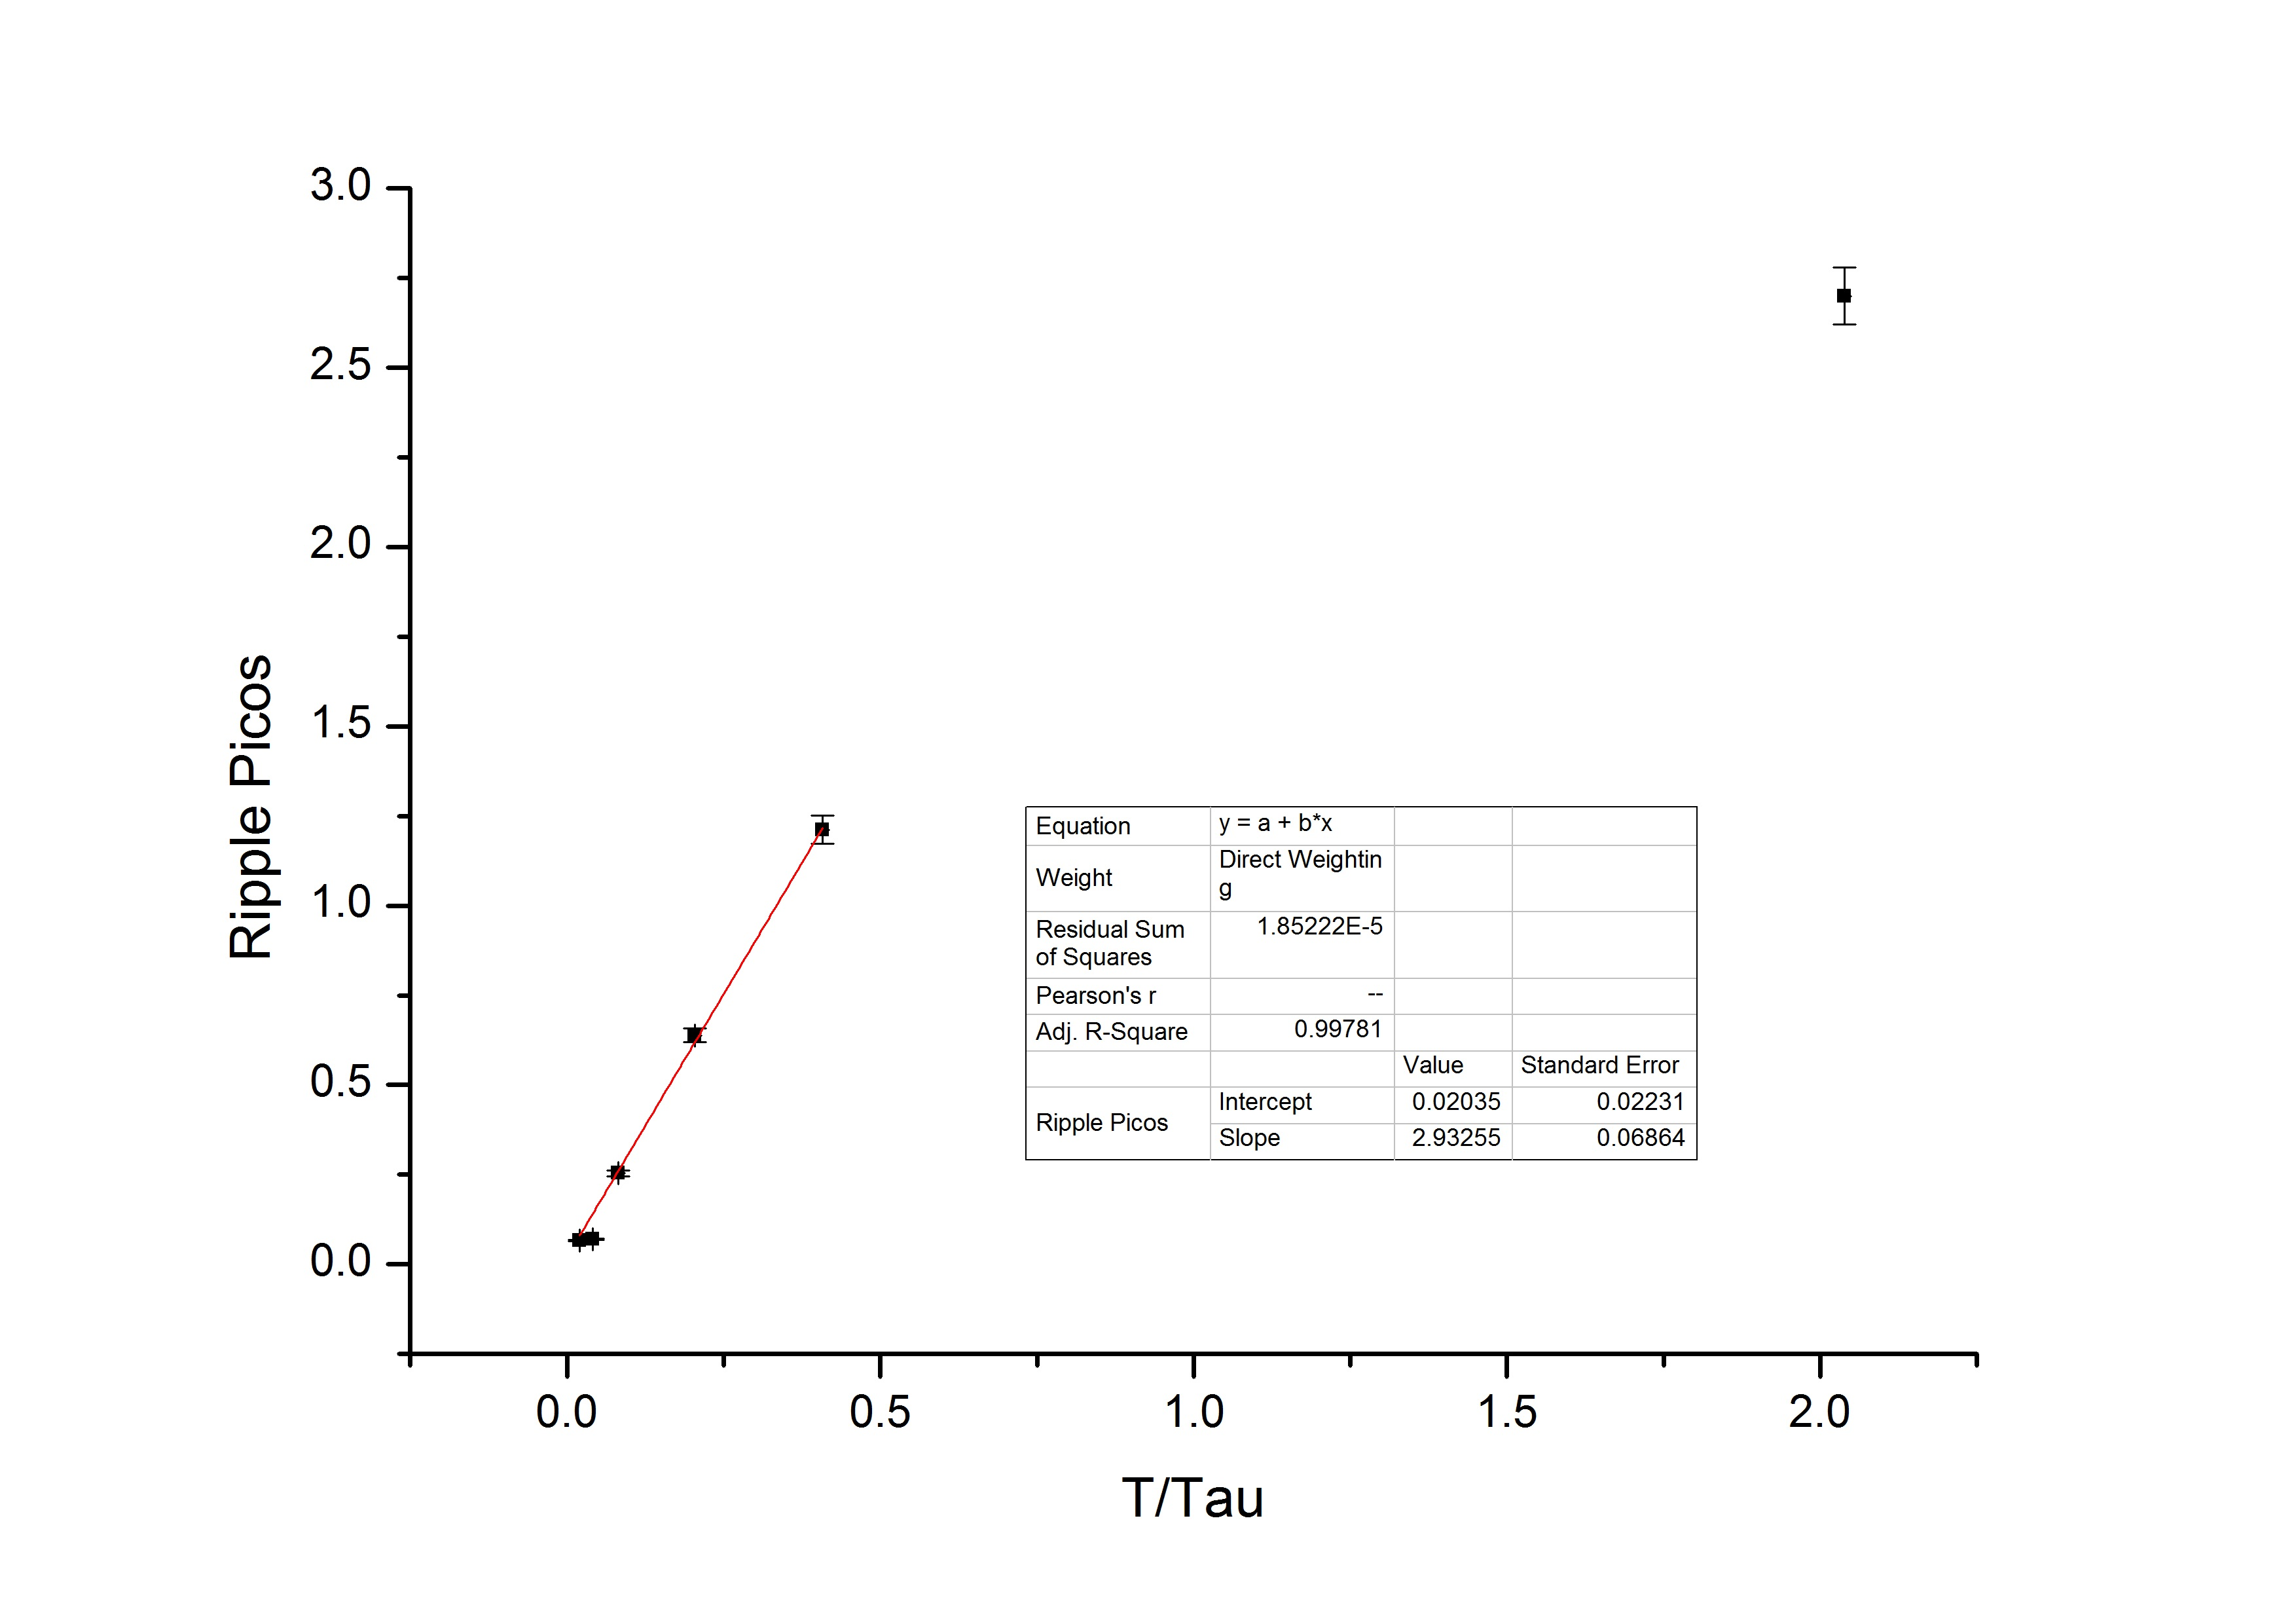
\includegraphics[scale=0.35]{Ripple_Picos}
  \caption{Relación entre $\frac{T}{\tau}$ y las mediciones de ripple obtenidas promediando picos.}
  \label{subfig:picos}
\end{subfigure}
\begin{subfigure}{0.5\textwidth}
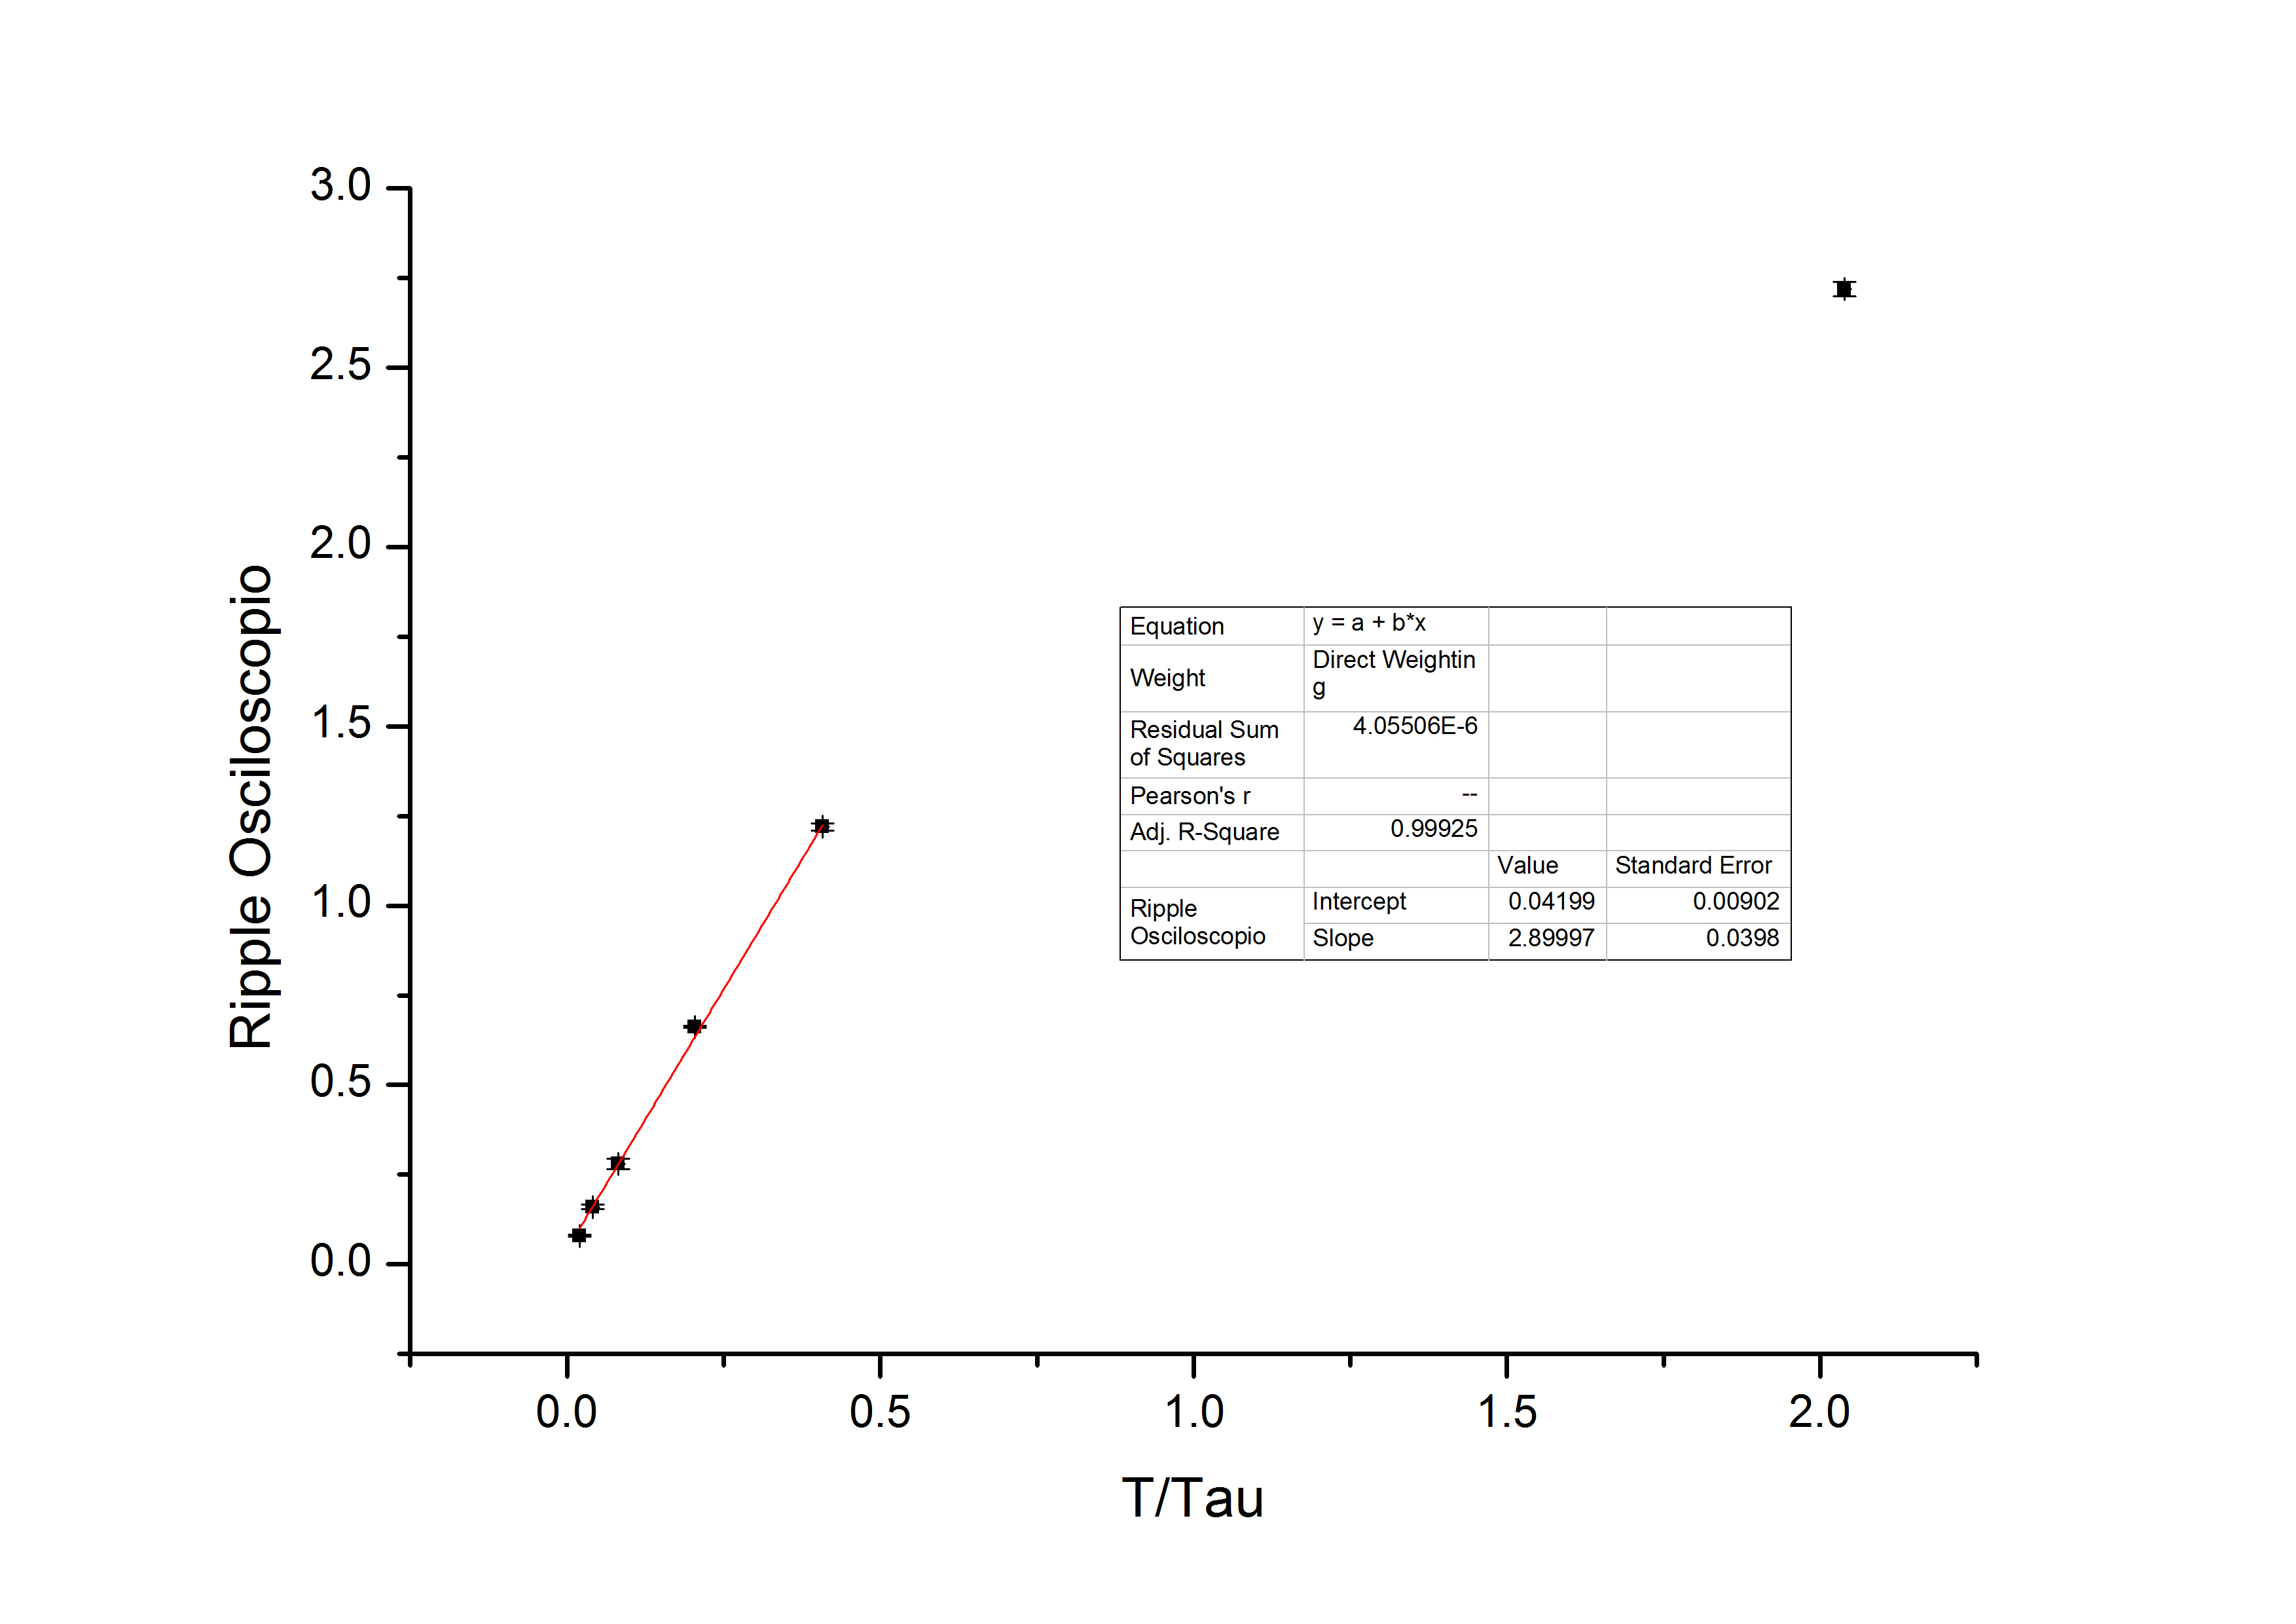
\includegraphics[scale=0.35]{Ripple_Osc}
  \caption{Relación entre $\frac{T}{\tau}$ y las mediciones de ripple obtenidas a través del osciloscopio}
  \label{subfig:osc}
\end{subfigure}
  \caption{Ripples en función de  $\frac{T}{\tau}$. El ajuste lineal es confiable para los primeros 4 puntos solamente en ambos casos}
  \label{fig:ripples_Tau}
\end{figure}

El ajuste lineal de \textbf{Figura \ref{subfig:picos}} arroja un $R_Square = 0.99781$ con una pendiente $m_p = (2.93 \pm 0.07)V$ y ordenada $b_p = (0.02 \pm 0.02)V$ mientras que el de la \textbf{Figura \ref{subfig:osc}} arroja un $R_Square = 0.99925$ con una pendiente $m_o = (2.90 \pm 0.04)V$ y ordenada $b_o = (0.042 \pm 0.009)V$. Tanto las pendientes como las ordenadas resultan indistinguibles dentro del error. 


\subsubsection{Rectificador de onda completa}
Para esta sección, el análisis fue mucho más veloz tras haber concluído que los valores arrojados por el osciloscopio resultaban indistinguibles de los arrojados por el análisis, por lo que no era necesario el esfuerzo adicional. Los ripples obtenidos a través del osciloscopio para las distintas resistencias pueden verse en la \textbf{Figura \ref{fig:ripples_completa}}.

\begin{figure}[h]
\centering
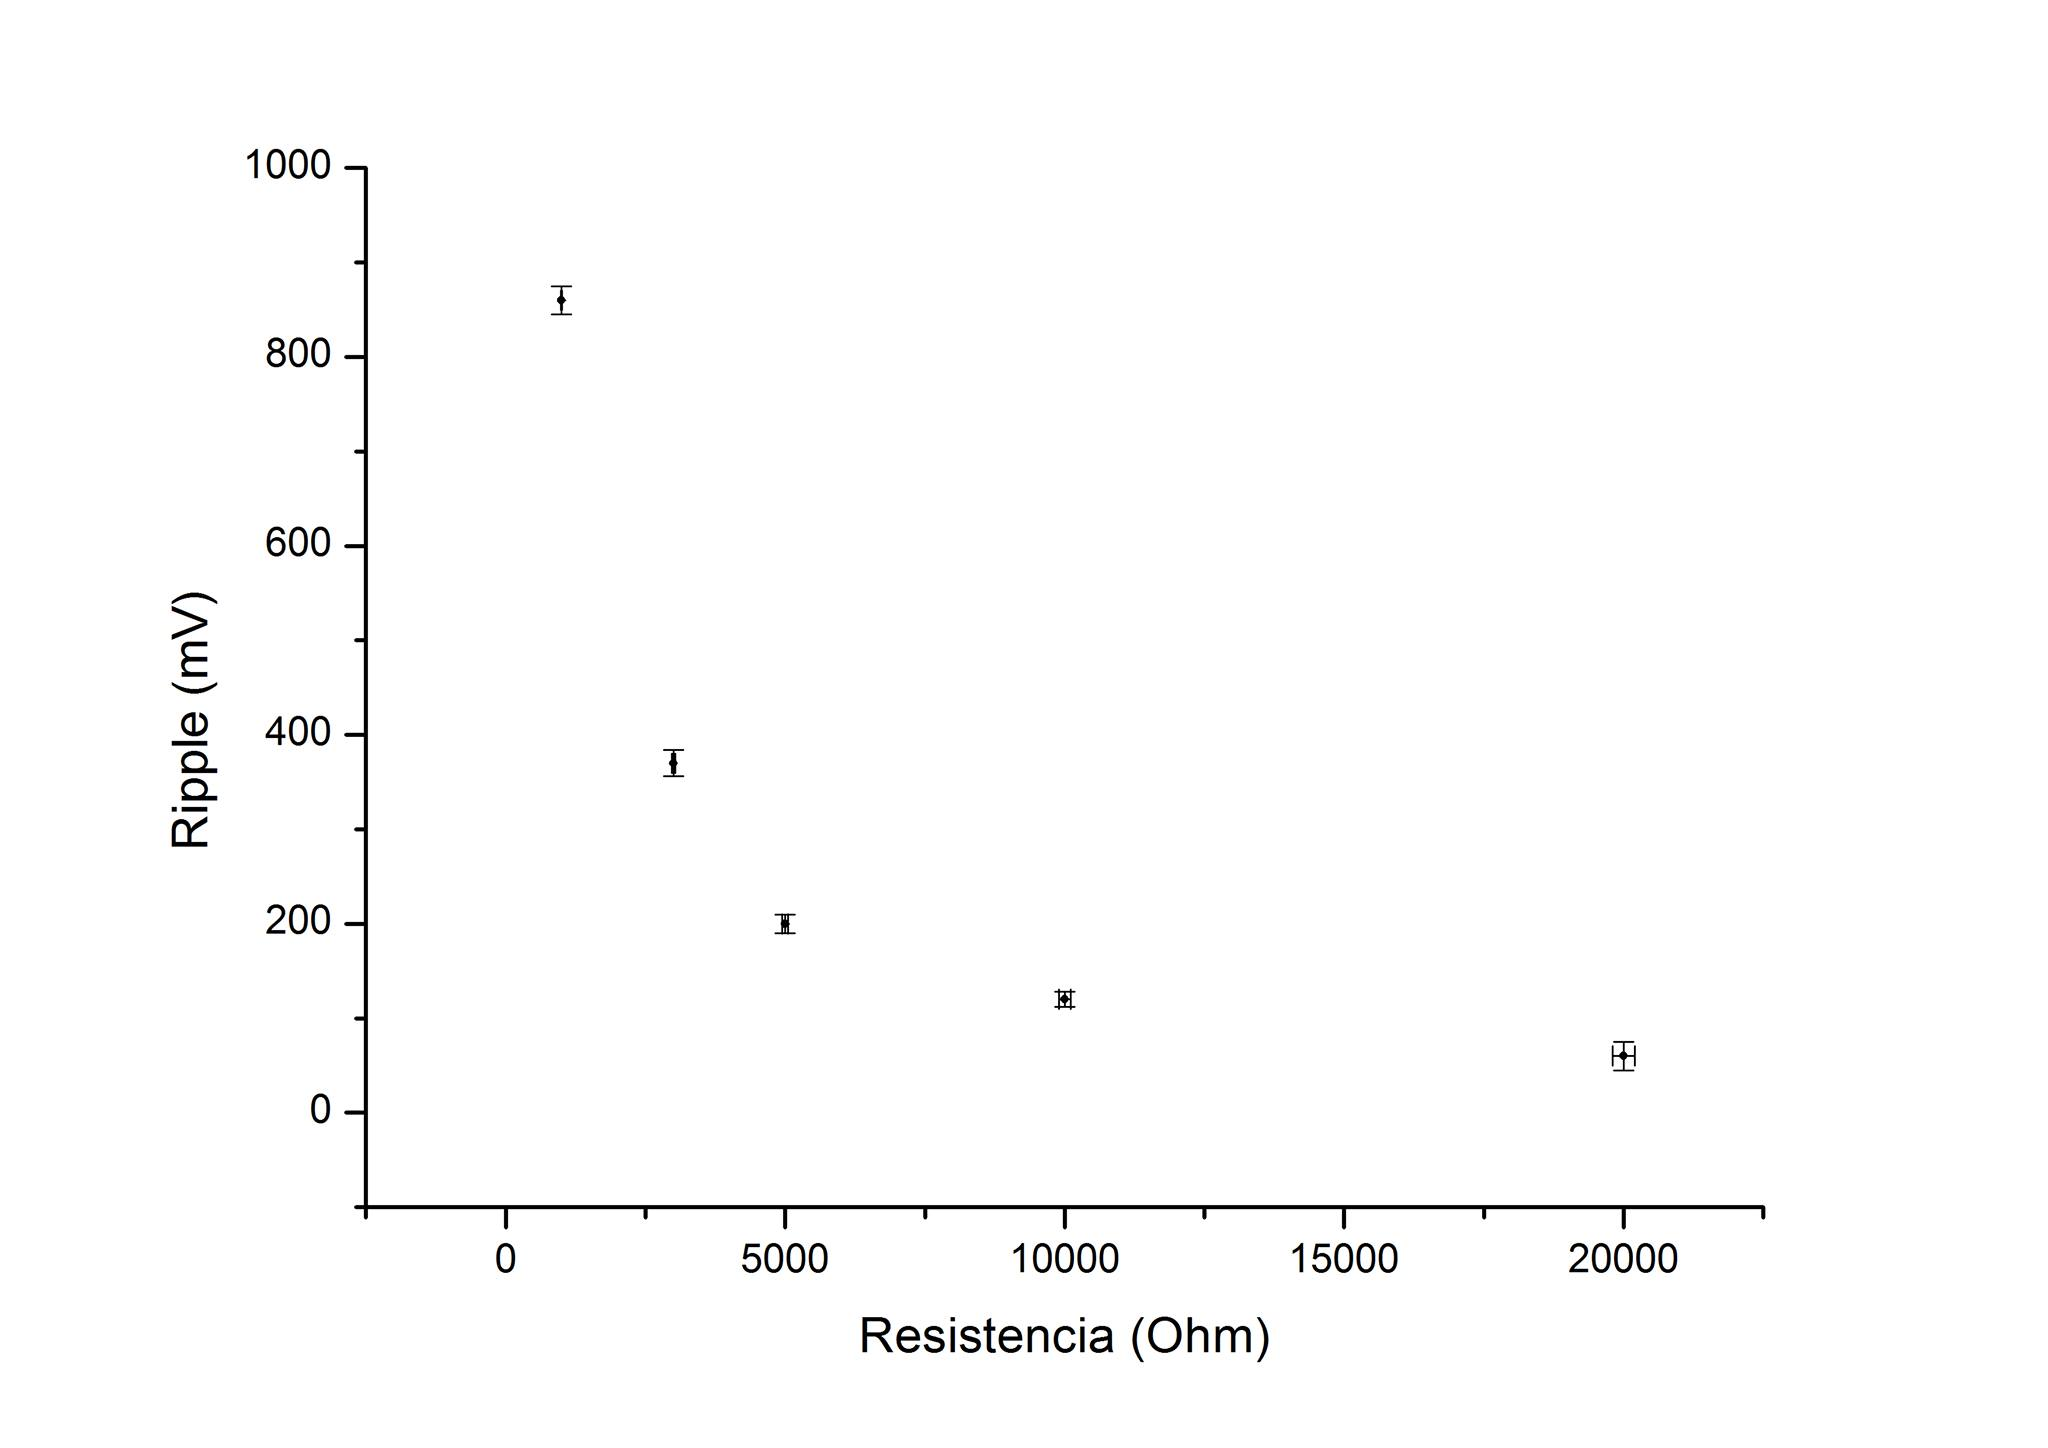
\includegraphics[scale=0.18]{ripples_completa}
   \caption{Relación de los ripples medidos directamente del osciloscopio y la resistencia utilizada.}
   \label{fig:ripples_completa}
\end{figure}

Nuevamente, se graficaron los riples en función de $\frac{T}{\tau}$ donde $T = (20.000 \pm 0.002)ms$ y nuevamente $\tau = RC$, obteniendo el gráfico de la \textbf{Figura \ref{fig:completa_lineal}}. El ajuste lineal arroja un $R-Square = 0.98897$ que asegura la bondad del ajuste junto con una pendiente $m = (0.41 \pm 0.02)V$ y una ordenada $b = (0.04 \pm 0.02)V$. 

\begin{figure}[h]
\centering
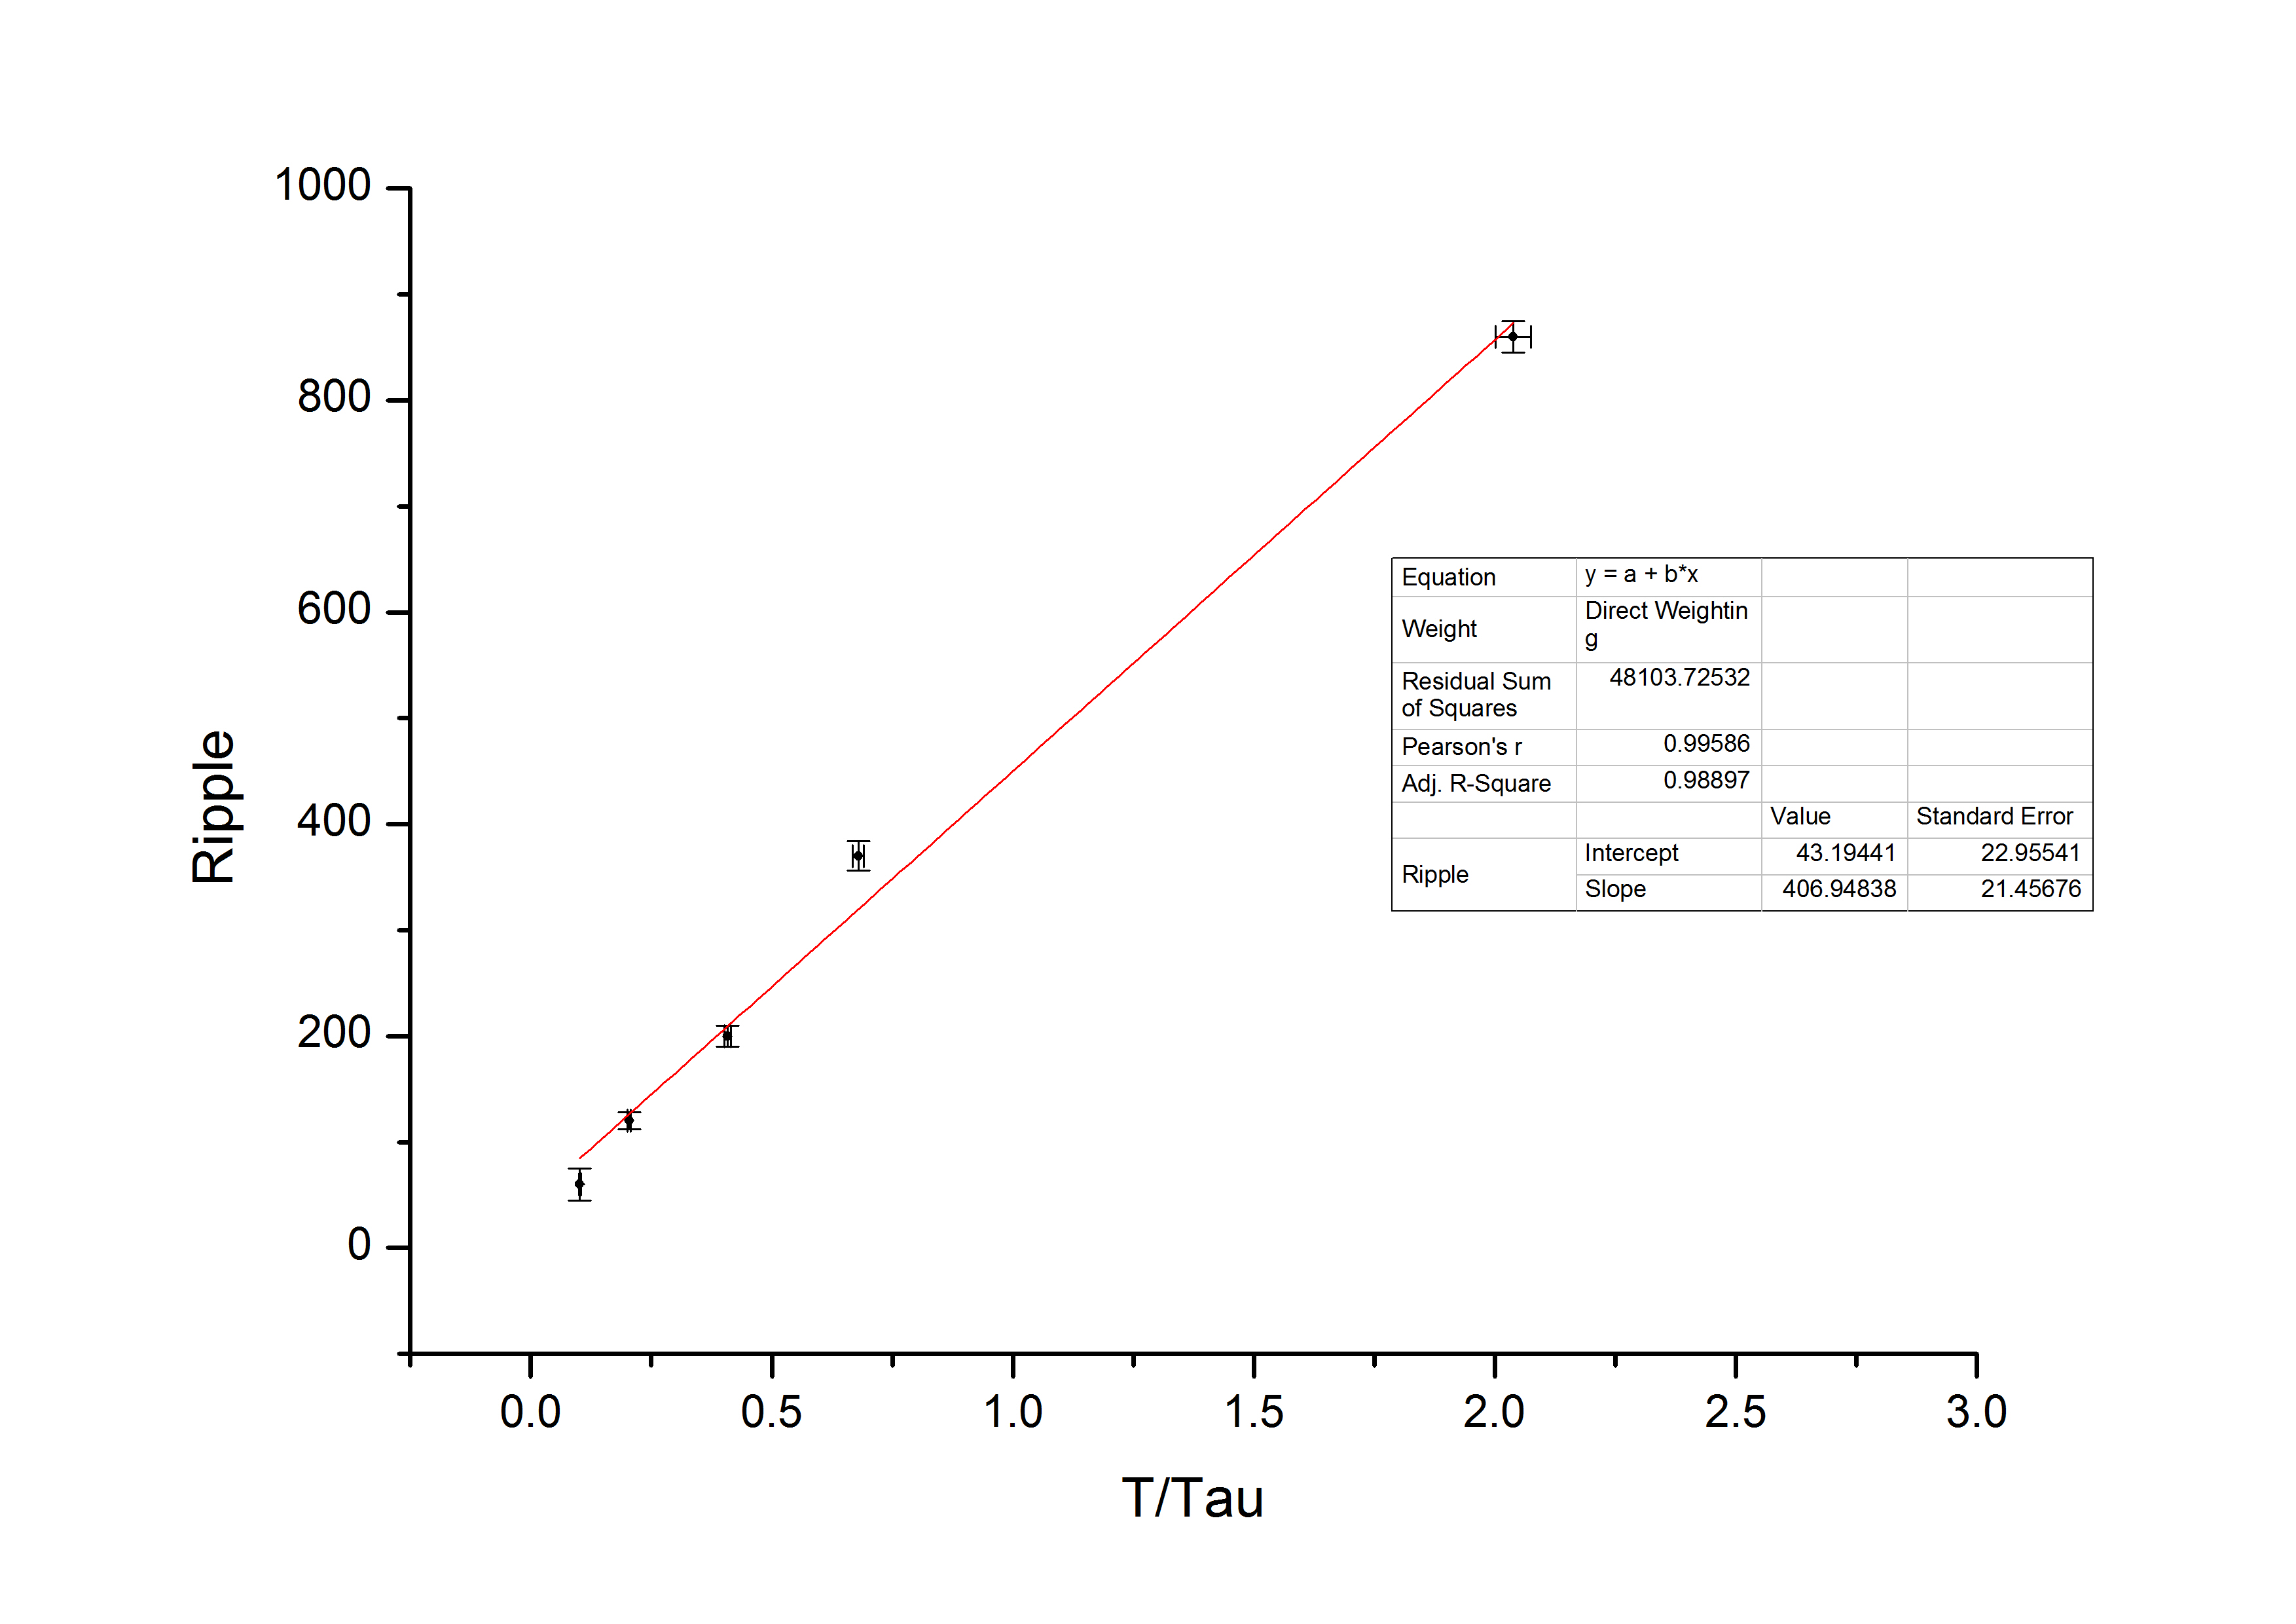
\includegraphics[scale=0.37]{completa_lineal}
   \caption{Relación de los ripples medidos y $\frac{T}{\tau}$. El ajuste lineal es preciso para todo el rango de valores manejado}
   \label{fig:completa_lineal}
\end{figure}

%%%%%%%%%%%%%%%%%%%%%%%%%%%%%%%%%%%%%%%%%%%%%%%%%%%%%%%%%%%%%%%%%%%%%%%%%%%%%%%%%%%%%%%%%%%%%%%%%%%%%%%%%%%%%%%%%%%%%%%%%%%%%%%%
%	CONCLUSIONES
%%%%%%%%%%%%%%%%%%%%%%%%%%%%%%%%%%%%%%%%%%%%%%%%%%%%%%%%%%%%%%%%%%%%%%%%%%%%%%%%%%%%%%%%%%%%%%%%%%%%%%%%%%%%%%%%%%%%%%%%%%%%%%%%

\section{Conclusiones}

Los resultados obtenidos durante la caracterización de diodos, aunque sean consistentes con lo esperado, no resultan confiables debido a que los coeficientes $R-Square$ no son tan cercanos a 1. En particular, al no conocer los parametros
realmente los parámetros para caracterizar los diodos no hubo oportunidad de constrastar los resultados. El principal motivo de desconfianza es que los coeficientes $R-Square$ resultan bajos en todos los ajustes aun cuando la cantidad
de puntos ajustados es relativamente pequeña (entre 4 y 7 puntos). Esto puede deberse a que el método utilizado a la hora de analizar los datos en un intento por reducir las fluctuaciones de las curvas iniciales (como puede verse en la 
\textbf{figura \ref{fig:simple_feo}}) no fue suficiente o correcto, quizás debido al criterio utilizado para fijar los $CT$. En definitiva, aunque el método utilizado fue muy veloz y sencillo a la hora de realizar las mediciones, acarreo
una gran cantidad de problemas a la hora de analizar los datos. No obstante, pudieron verse y comprobarse con cierta confiabilidad que los diodos evitan el paso de corriente hasta llegar a un voltaje límite, a partir del cual actua en
forma similar a una resistencia siguiendo \eqref{Aprox}. Para el caso particular del Zenek pudo observarse el efecto avalancha para corriente en inversa.

Respecto a los rectificadores, la comprobación de que los valores arrojados por el osciloscopio y los obtenidos mediante analisis de picos son indistinguibles no es un dato menor, aunque sea esperable. Principalmente esto significa que
la forma de operar del osciloscopio debe ser igual o mejor que el análisis de picos realizados a pesar de hacerlo en el momento. Concentrandose más en el rectificador en si, se pudo comprobar que la magnitud importante a la hora de
rectificar la señal es la relación entre el período de la señal y el período de carga del capacitor gracias a las \textbf{Figuras \ref{fig:ripples_Tau}} y \textbf{\ref{fig:completa_lineal}}. En particular, se pudo comprobar una cierta
linealidad para valores de $\frac{T}{\tau}$ bajos (menores a 1) con los Ripples en un rectificador de media onda gracias a los ajustes realizados sobre \textbf{Figura \ref{subfig:picos}} y \textbf{\ref{subfig:osc}} arroja un par de 
$R_Square = 0.99781$ y $R_Square = 0.99925$ con pendientes indistinguibles $m_p = (2.93 \pm 0.07)V$ y $m_o = (2.90 \pm 0.04)V$, respectivamente. Esto comprueba con bastante confiabilidad la linealidad de la relación. Para el rectificador
de onda completa, la linealidad pudo verse en todos los valores de $\frac{T}{\tau}$ medidos gracias al ajuste sobre la \textbf{Figura \ref{fig:completa_lineal}} que arrojó un $R-Square = 0.98897$, por lo que a priori podría suponerse que en
el rectificador de onda completa la relación es aproximadamente lineal para valores de $\frac{T}{\tau}$ mayores que en el de media onda. Sin embargo, cabe aclarar que se desconoce el significado de estas pendientes o la relación que
puedan tener con los parámetros.
\label{sec:conclusiones}




%%%%%%%%%%%%%%%%%%%%%%%%%%%%%%%%%%%%%%%%%%%%%%%%%%%%%%%%%%%%%%%%%%%%%%%%%%%%%%%%%%%%%%%%%%%%%%%%%%%%%%%%%%%%%%%%%%%%%%%%%%%%%%%%%
%	APÉNDICE: esas cosas extras que simplemente no tuvieron lo suficiente como para ganarse una sección propia.
%%%%%%%%%%%%%%%%%%%%%%%%%%%%%%%%%%%%%%%%%%%%%%%%%%%%%%%%%%%%%%%%%%%%%%%%%%%%%%%%%%%%%%%%%%%%%%%%%%%%%%%%%%%%%%%%%%%%%%%%%%%%%%%%%



%%%%%%%%%%%%%%%%%%%%%%%%%%%%%%%%%%%%%%%%%%%%%%%%%%%%%%%%%%%%%%%%%%%%%%%%%%%%%%%%%%%%%%%%%%%%%%%%%%%%%%%%%%%%%%%%%%%%%%%%%%%%%%%%%
%	REFERENCIAS: libros, libros, libros.
%%%%%%%%%%%%%%%%%%%%%%%%%%%%%%%%%%%%%%%%%%%%%%%%%%%%%%%%%%%%%%%%%%%%%%%%%%%%%%%%%%%%%%%%%%%%%%%%%%%%%%%%%%%%%%%%%%%%%%%%%%%%%%%%%

%Ejemplo:
%\begin{thebibliography}{1}
 %\bibitem{Berkeley} Frank S. Crawford, \textit{Berkeley physics course 3: Ondas}, 1994, Editorial Reverte S.A.
%\end{thebibliography}
%Para citar: blablabla \cite{Baird}
 
\end{document}





